
\documentclass[aspectratio=169,t]{beamer}

\usepackage[T1]{fontenc}
\usepackage{amsmath,amssymb}
\usepackage[sfdefault]{carlito}
\usepackage{coppecolor}
\graphicspath{{figs/}{logos/}}

\setbeamertemplate{navigation symbols}{}
\setbeamersize{text margin left=8mm,text margin right=8mm}
\setbeamercolor{normal text}{fg=coppeGraphite}
\setbeamercolor{structure}{fg=coppeAccent}
\setbeamerfont{frametitle}{size=\large}
\setbeamertemplate{frametitle}{%
  \vspace*{4mm}{\color{coppeGraphite}\MakeUppercase{\insertframetitle}}\par\vspace{1mm}%
  {\color{coppeAccent}\rule{10mm}{0.8mm}}\par}
\setbeamertemplate{footline}{%
  \hspace*{8mm}\raisebox{2mm}{
\includegraphics[height=4.5mm]{COPPE-LOGO-PNG}}\hfill
  \raisebox{3mm}{\tiny\color{coppeGray}\insertframenumber\,/\,\inserttotalframenumber}\hspace*{8mm}}

% Cores por papel: gerador, discriminador
\newcommand{\cG}[1]{\textcolor{coppeAccent}{#1}}
\newcommand{\cD}[1]{\textcolor{coppeWine}{#1}}
% Bloco de rótulo com barra colorida, da altura do trecho da figura ao lado
\newcommand{\bloco}[4]{\noindent{\color{#1}\rule{0.7mm}{#2}}\hspace{2mm}%
  \parbox[b][#2][c]{55mm}{{\small\textcolor{#1}{\textbf{#3}}}\par\smallskip{\footnotesize #4}}\par\vspace{0.5mm}}
% Credito da figura, embaixo, sem TikZ: nao exige segunda passada
\newcommand{\fonte}[1]{\par\vfill\raggedright{\tiny\color{coppeGray}#1\par}}

\begin{document}

\begin{frame}[plain]
  \begin{minipage}[t][80mm][t]{\textwidth}
    \vspace{3mm}
    {\small\textbf{CPE727 \textperiodcentered{} Aprendizado Profundo}}\hfill
    \raisebox{-7mm}{
\includegraphics[height=10mm]{logo_peb}\hspace{4mm}
\includegraphics[height=10mm]{COPPE-LOGO-PNG}}\par
    {\footnotesize\color{coppeGray}COPPE, Universidade Federal do Rio de Janeiro\par}
    \vfill
    {\fontsize{24}{28}\selectfont Redes Adversárias Generativas (GANs)\par}
    \vspace{3mm}
    {\color{coppeAccent}\rule{13mm}{1.2mm}\par}
    \vspace{3mm}
    \parbox{130mm}{\small\color{coppeGray}Seminário 8. Como funcionam, por que é difícil treinar, StyleGAN, Pix2Pix e CycleGAN. Goodfellow, cap. 20}
    \vfill
    {\footnotesize\textbf{Pedro Henrique Batista Campos \textperiodcentered{} Daniel Cordeiro Marques}}\hfill
    {\footnotesize\color{coppeGray}12 de novembro de 2026}
  \end{minipage}
\end{frame}
\section{Introdução}

\begin{frame}{O que vamos ver}
  \centering
  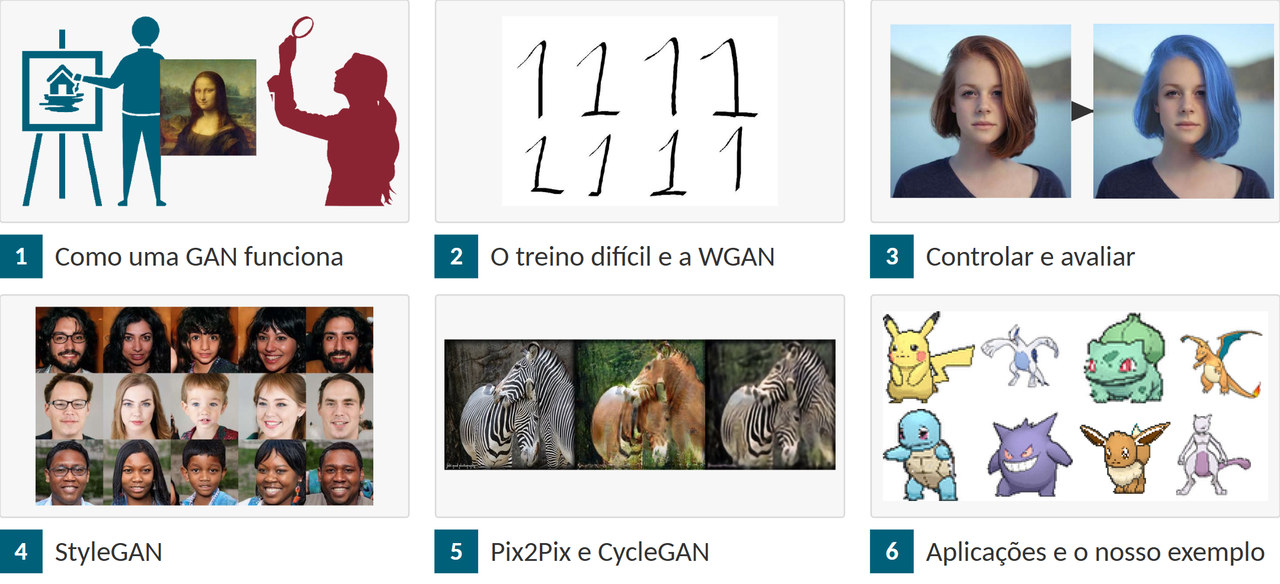
\includegraphics[width=124.4mm]{f_mapa}
  \fonte{Imagens: DeepLearning.AI \textperiodcentered{} sprites: Zhang et al., Dive into Deep Learning}
\end{frame}

\begin{frame}{De borrões a rostos}
  \centering
  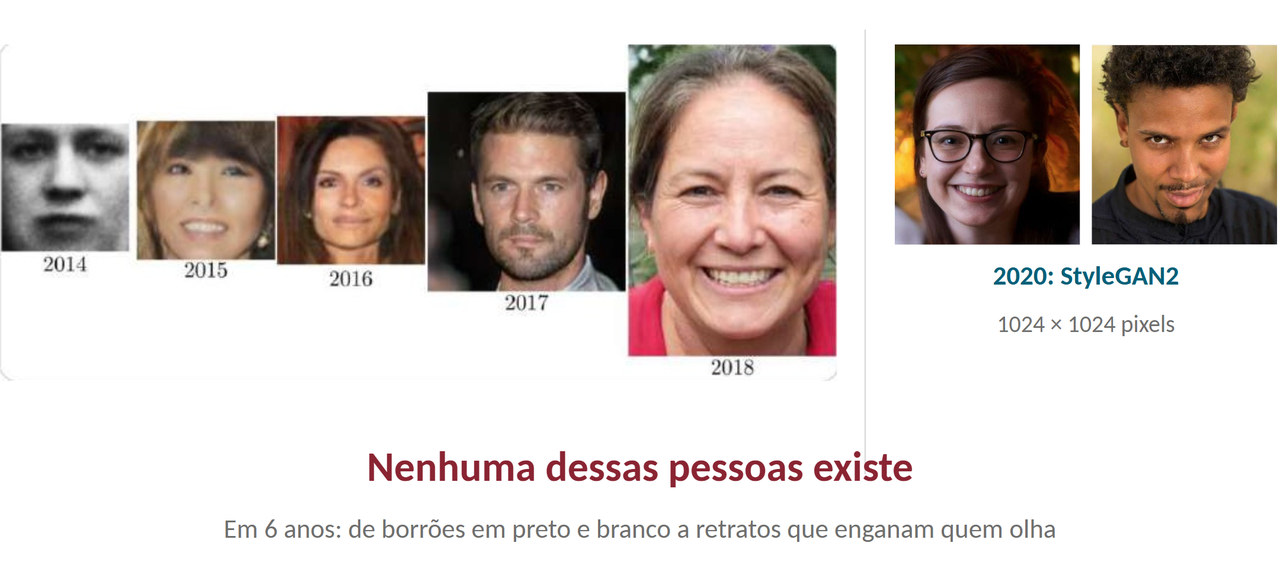
\includegraphics[width=124.4mm]{f_evolucao}
  \fonte{Tweet de I. Goodfellow, em DeepLearning.AI C2W3 \textperiodcentered{} StyleGAN2: Karras et al. 2020, em C1W1}
\end{frame}

\begin{frame}{Roteiro}
  \vspace{4mm}
    {\small\textcolor{coppeAccent}{\textbf{1. Como uma GAN funciona}}}\par\smallskip
    {\footnotesize\textcolor{coppeGray}{O jogo, a matemática e a primeira GAN de imagem}}\par\smallskip
    {\small\textcolor{coppeGray}{{2. Problemas na dinâmica adversarial}}}\par\smallskip
    {\small\textcolor{coppeGray}{{3. Controlar e avaliar}}}\par\smallskip
    {\small\textcolor{coppeGray}{{4. StyleGAN}}}\par\smallskip
    {\small\textcolor{coppeGray}{{5. Pix2Pix e CycleGAN}}}\par\smallskip
    {\small\textcolor{coppeGray}{{6. Aplicações e o nosso exemplo}}}\par\smallskip
\end{frame}

\begin{frame}{Discriminativo e generativo}
  \centering
  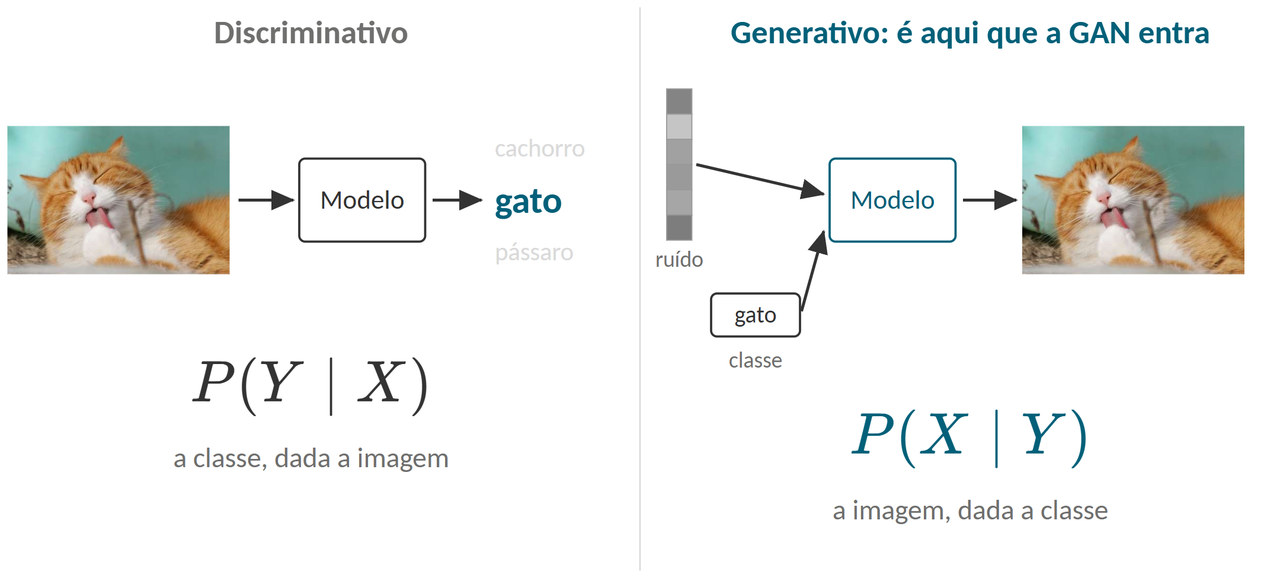
\includegraphics[width=124.4mm]{f_gd}
  \fonte{Adaptado de DeepLearning.AI C1W1 \textperiodcentered{} Goodfellow cap. 20}
\end{frame}

\begin{frame}{A ideia: pintor contra detetive}
  \centering
  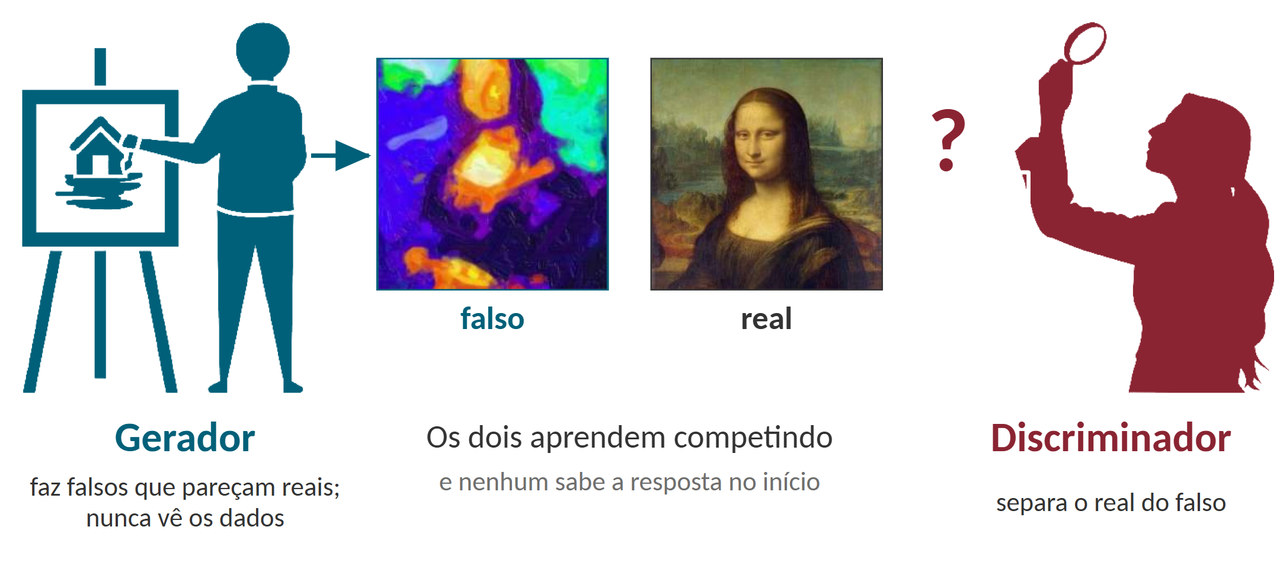
\includegraphics[width=124.4mm]{f_ideia}
  \fonte{Silhuetas e imagens: DeepLearning.AI C1W1 \textperiodcentered{} Goodfellow et al. 2014}
\end{frame}
\section{Dinâmica adversarial}

\begin{frame}{O jogo}
  \centering
  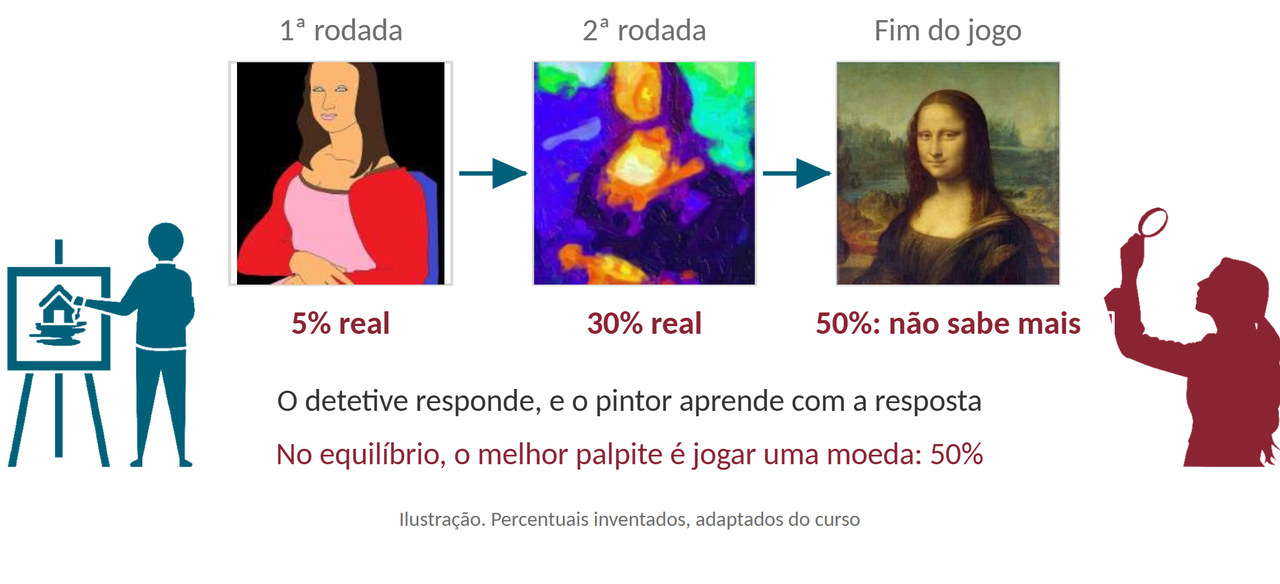
\includegraphics[width=124.4mm]{f_jogo}
  \fonte{Adaptado de DeepLearning.AI C1W1}
\end{frame}

\begin{frame}{O discriminador}
  \centering
  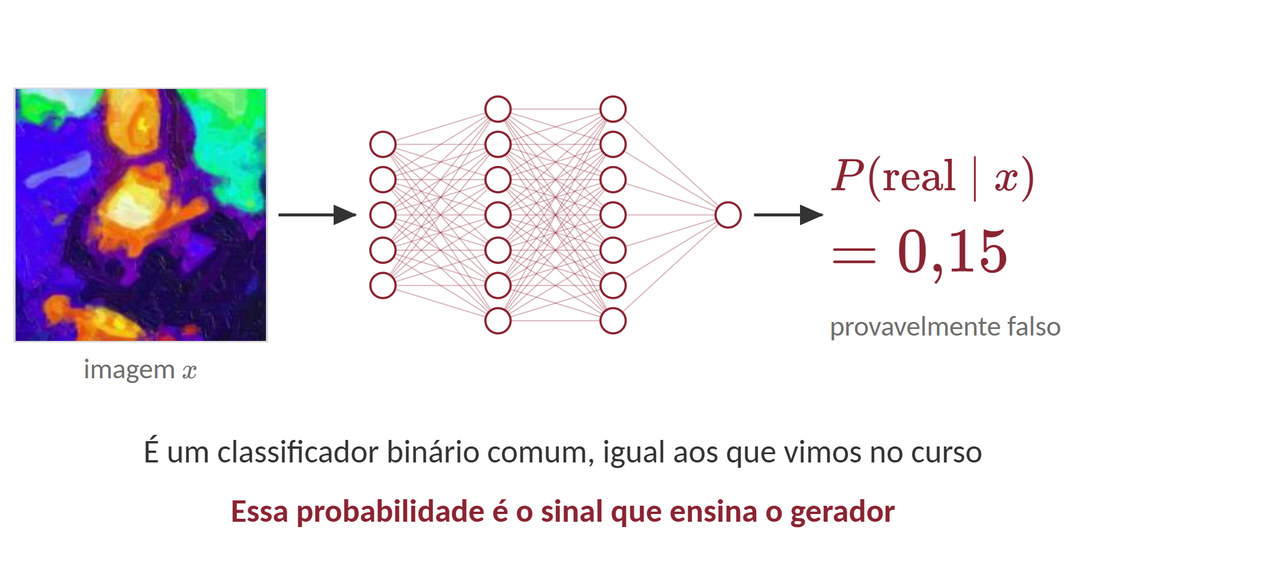
\includegraphics[width=124.4mm]{f_disc}
  \fonte{Adaptado de DeepLearning.AI C1W1}
\end{frame}

\begin{frame}{O gerador}
  \centering
  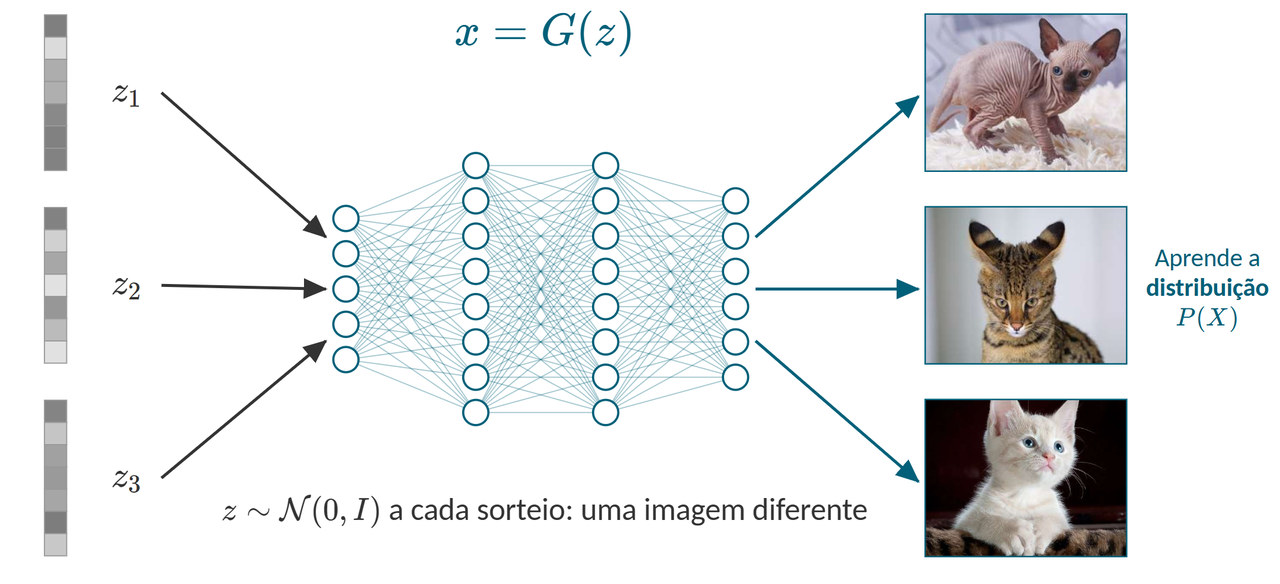
\includegraphics[width=124.4mm]{f_ger}
  \fonte{Adaptado de DeepLearning.AI C1W1 \textperiodcentered{} Goodfellow eq. 20.71}
\end{frame}

\begin{frame}{O custo: entropia cruzada binária}
  \centering
  \resizebox{93.3mm}{!}{$\displaystyle J(\theta)=-\frac{1}{m}\sum_{i=1}^{m}\Big[\underbrace{y^{(i)}\log h(x^{(i)},\theta)}_{\text{conta quando }y=1}+\underbrace{(1-y^{(i)})\log\big(1-h(x^{(i)},\theta)\big)}_{\text{conta quando }y=0}\Big]$}\par\vspace{1.5mm}
  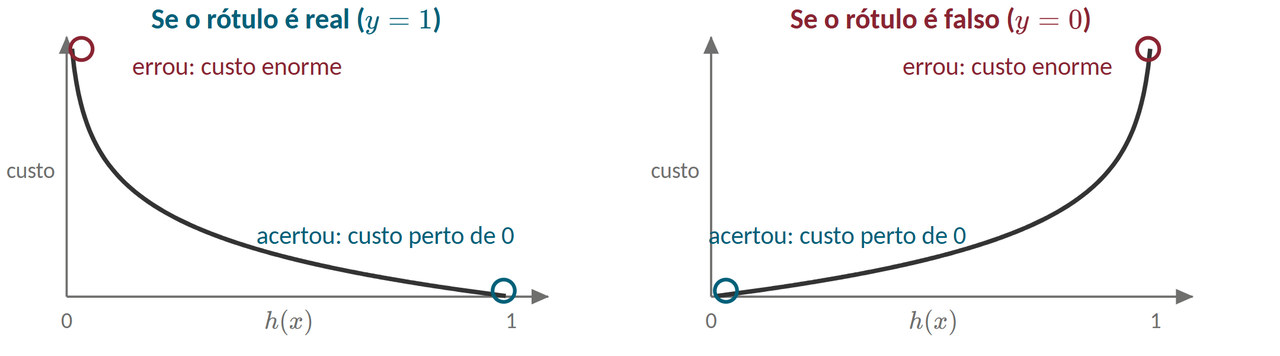
\includegraphics[width=124.4mm]{f_bce}
  \fonte{DeepLearning.AI C1W1}
\end{frame}

\begin{frame}{Treino: o passo do discriminador}
  \centering
  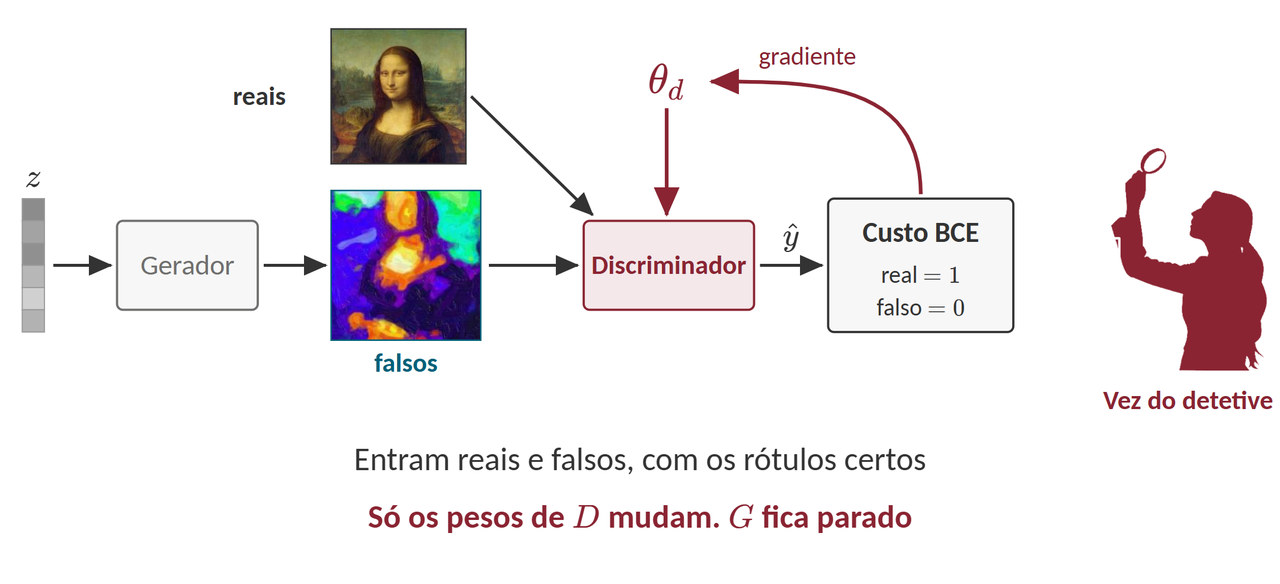
\includegraphics[width=124.4mm]{f_passo_d}
  \fonte{Adaptado de DeepLearning.AI C1W1}
\end{frame}

\begin{frame}{Treino: o passo do gerador}
  \centering
  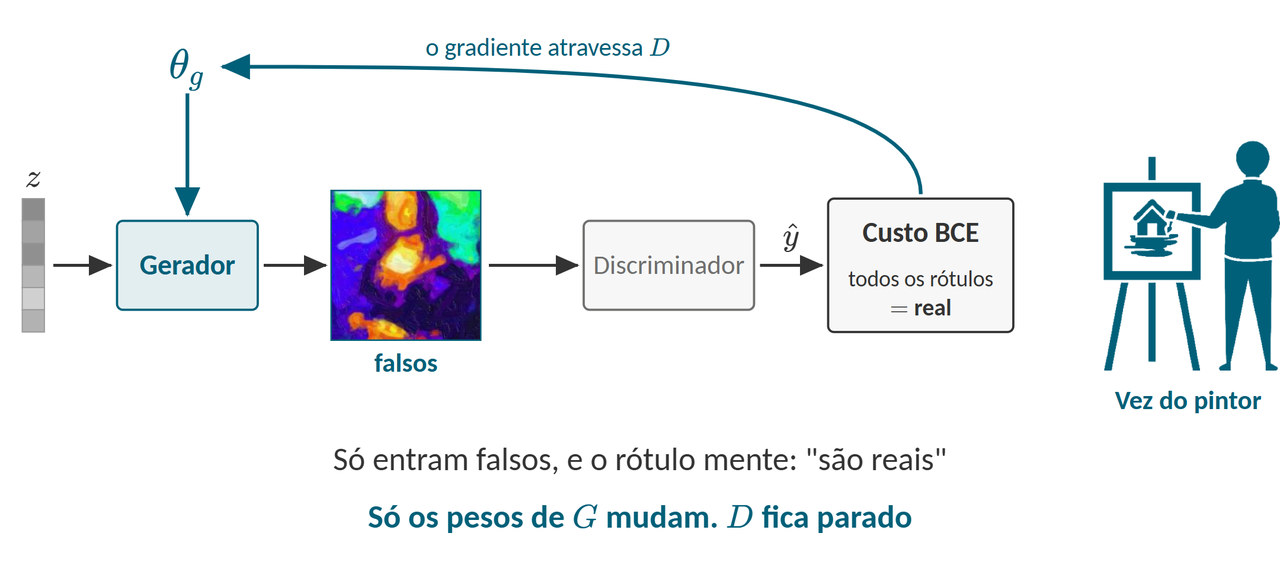
\includegraphics[width=124.4mm]{f_passo_g}
  \fonte{Adaptado de DeepLearning.AI C1W1}
\end{frame}

\begin{frame}{O jogo em uma equação}
  \centering
  \resizebox{99.4mm}{!}{$\displaystyle \min_{\cG{G}}\max_{\cD{D}}\ V(D,G)=\underbrace{\mathbb{E}_{x\sim p_{\text{dados}}}\big[\log \cD{D}(x)\big]}_{\text{D acerta o real}}+\underbrace{\mathbb{E}_{z\sim p_z}\big[\log\big(1-\cD{D}(\cG{G}(z))\big)\big]}_{\text{D rejeita o falso; G quer o contrário}}$}\par\vspace{1.5mm}
  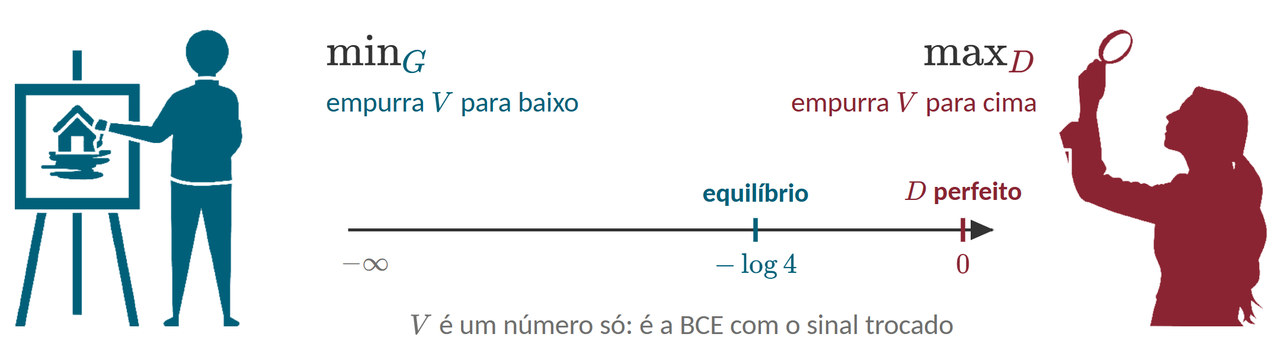
\includegraphics[width=124.4mm]{f_minimax}
  \fonte{Goodfellow eq. 20.80 e 20.81 \textperiodcentered{} Goodfellow et al. 2014, eq. 1}
\end{frame}

\begin{frame}{Custo não saturante}
  \centering
  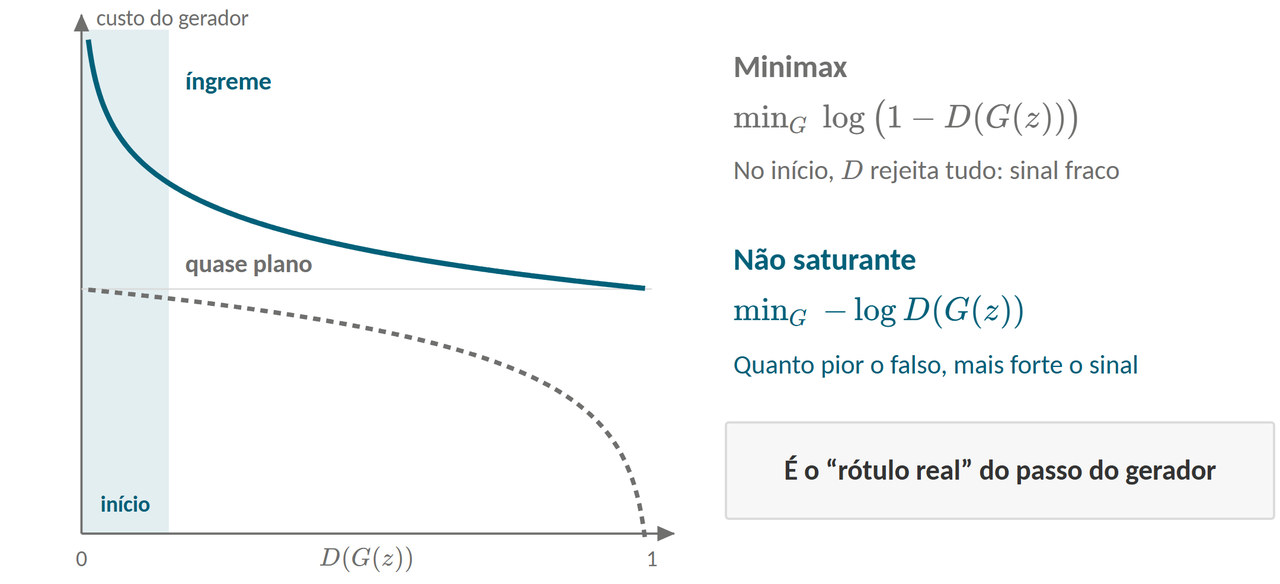
\includegraphics[width=124.4mm]{f_ns}
  \fonte{Goodfellow p. 701 \textperiodcentered{} tutorial de 2016, eq. 10 e 13 \textperiodcentered{} curvas calculadas}
\end{frame}

\begin{frame}{O melhor discriminador}
  \centering
  \resizebox{43.2mm}{!}{$\displaystyle D^{*}(x)=\frac{p_{\text{dados}}(x)}{p_{\text{dados}}(x)+p_g(x)}$}\par\vspace{1.5mm}
  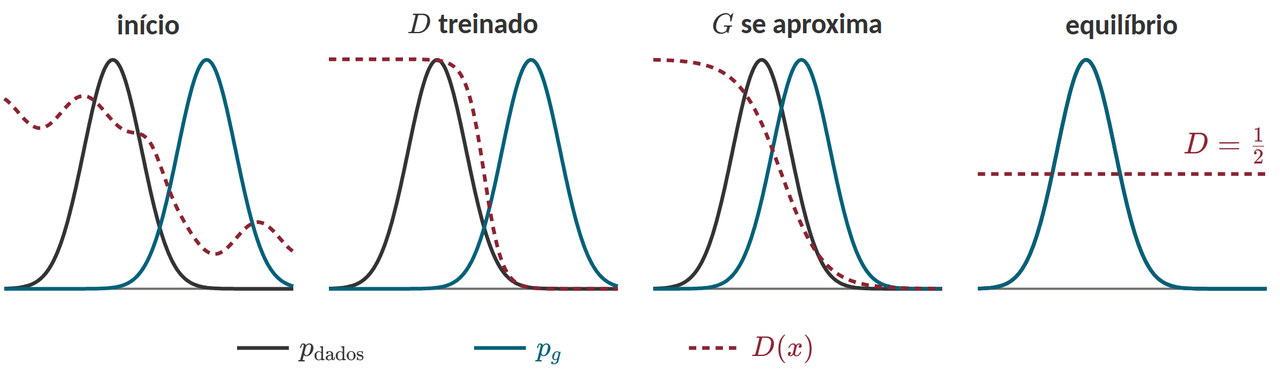
\includegraphics[width=124.4mm]{f_dotimo}
  \fonte{Goodfellow et al. 2014, prop. 1 e fig. 1 \textperiodcentered{} curvas calculadas}
\end{frame}

\begin{frame}{O que o gerador minimiza}
  \centering
  \resizebox{86.3mm}{!}{$\displaystyle \max_{D}V(D,G)=-\log 4+2\,\mathrm{JS}\big(p_{\text{dados}}\,\Vert\,p_g\big)\ \ge\ -\log 4$}\par\vspace{1.5mm}
  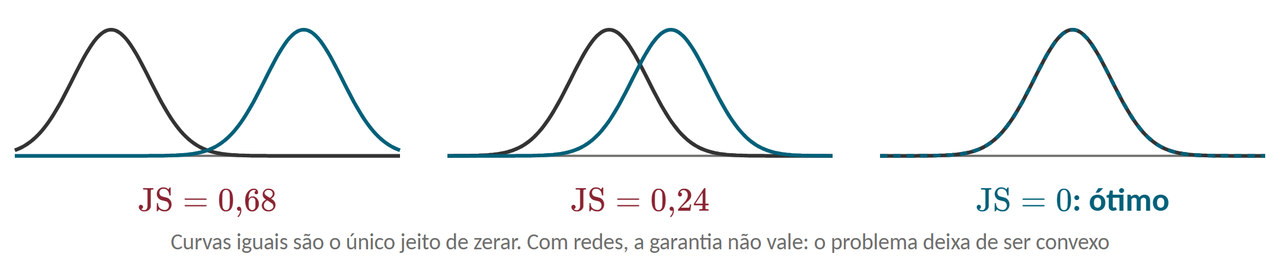
\includegraphics[width=124.4mm]{f_js}
  \fonte{Goodfellow et al. 2014, teo. 1 \textperiodcentered{} Goodfellow p. 700 \textperiodcentered{} JS calculada}
\end{frame}
\section{DCGAN}
\begin{frame}{DCGAN: GAN com convoluções}
  \centering
  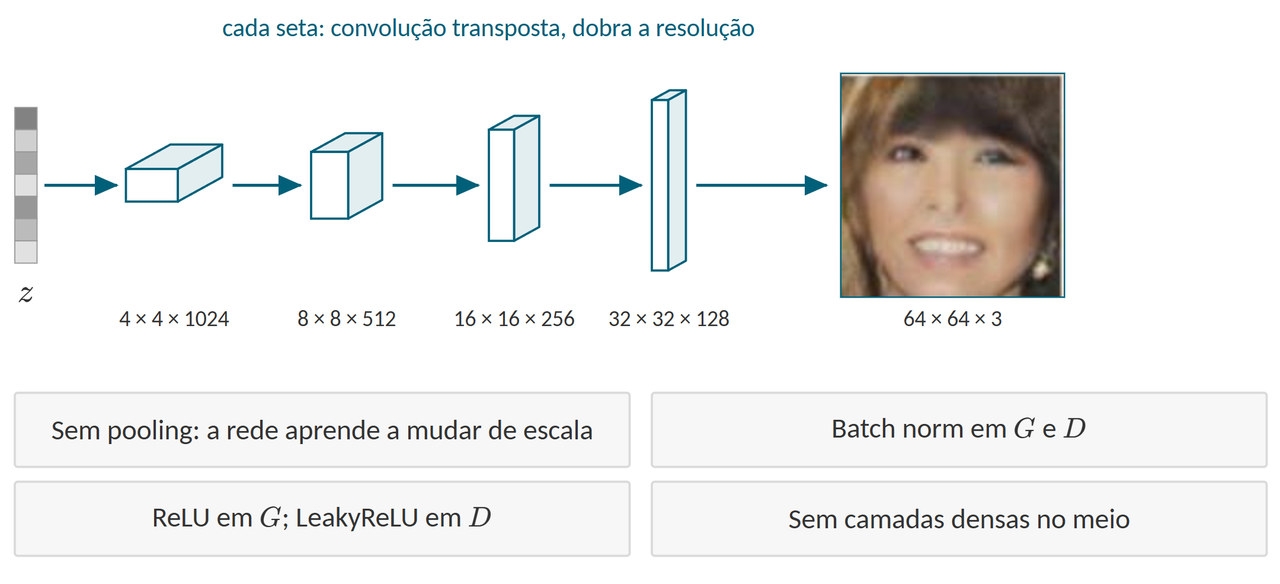
\includegraphics[width=124.4mm]{f_dcgan}
  \fonte{Radford et al. 2015, fig. 1 \textperiodcentered{} Goodfellow p. 701}
\end{frame}

\begin{frame}{DCGAN: o que ela gerou}
  \centering
  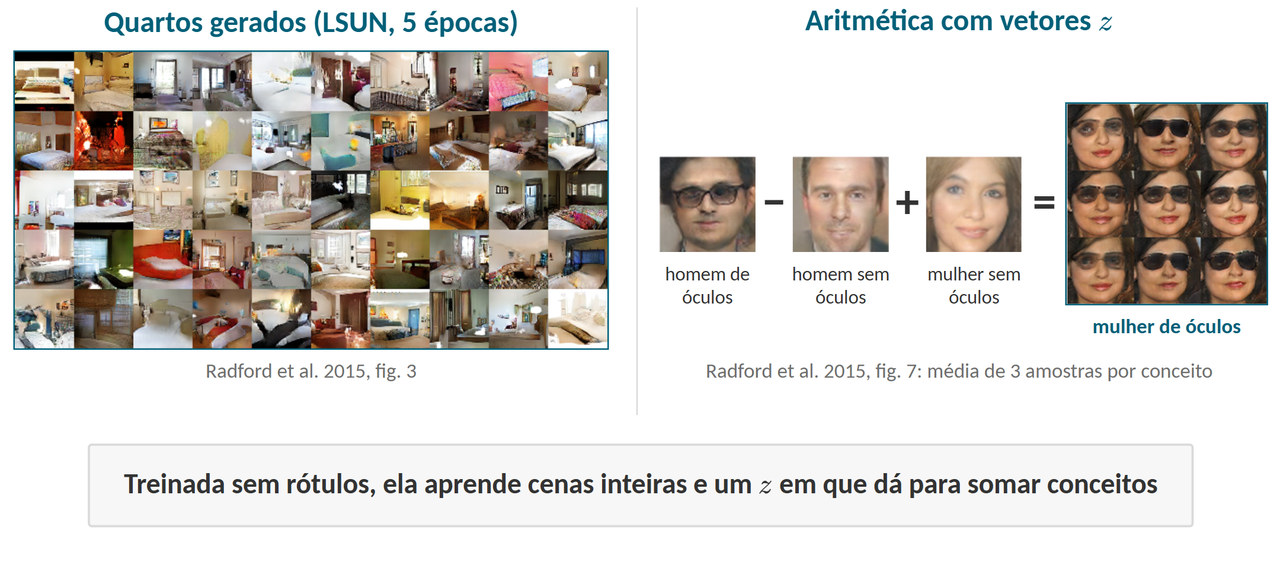
\includegraphics[width=124.4mm]{f_dcgan_casos}
  \fonte{Radford et al. 2015, fig. 3 e 7}
\end{frame}
\begin{frame}{Convolução transposta}
  \centering
  \resizebox{96mm}{!}{$\displaystyle o=\underbrace{s\,(i-1)}_{\text{onde começa a última contribuição}}+\underbrace{k}_{\text{tamanho do kernel}}-\underbrace{2p}_{\text{corta as bordas}}$}\par\vspace{1.5mm}
  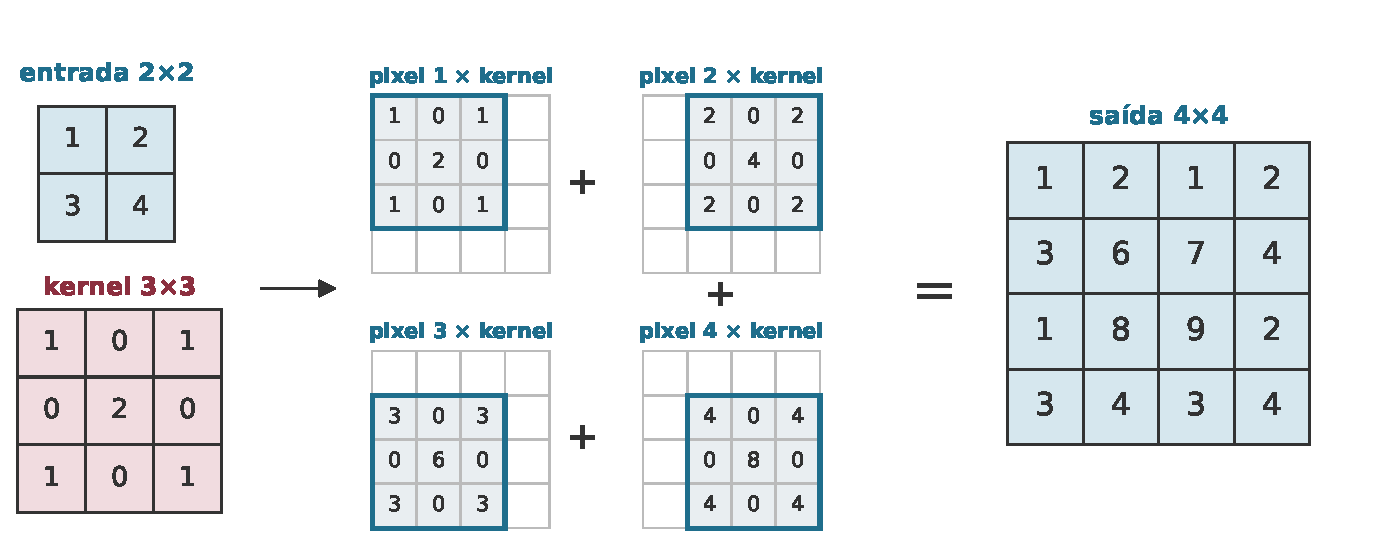
\includegraphics[width=124.4mm]{tc_carimbo}
  \fonte{Diagrama nosso \textperiodcentered{} Dumoulin e Visin 2016, seção 4 \textperiodcentered{} Radford et al. 2015}
\end{frame}

\begin{frame}{Artefatos de tabuleiro}
  \centering
    \begin{minipage}[c]{0.47\textwidth}\centering
    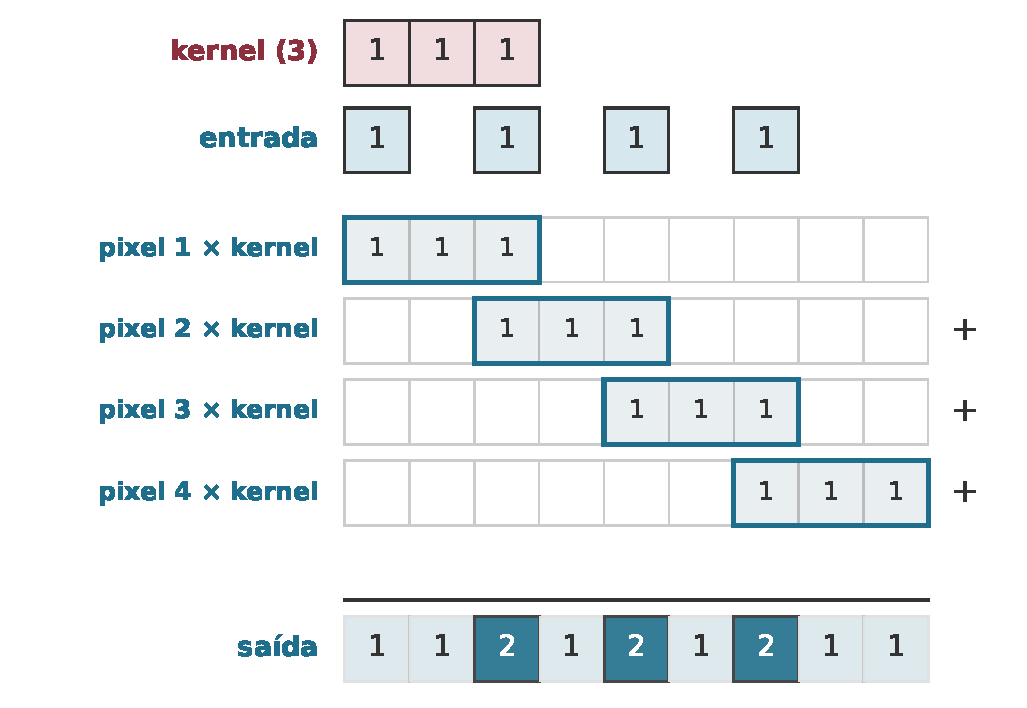
\includegraphics[width=\linewidth]{tab_k3}
  \end{minipage}\hfill
  \begin{minipage}[c]{0.5\textwidth}\centering
    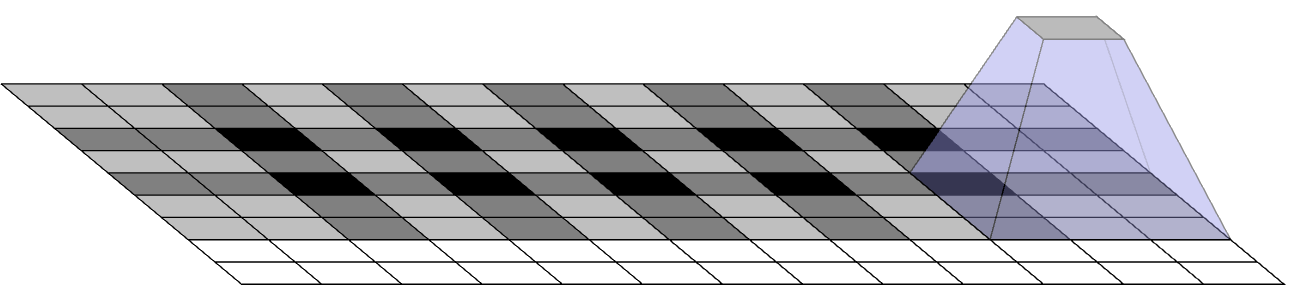
\includegraphics[width=\linewidth]{tab_1d}
  \end{minipage}
  \fonte{Diagrama nosso \textperiodcentered{} Odena, Dumoulin e Olah 2016, Distill}
\end{frame}

\begin{frame}{Como evitar esses artefatos?}
  \centering
  \begin{minipage}[t]{0.48\textwidth}\centering
    {\small\cG{\textbf{Redimensionar e convoluir}}}\par\smallskip
    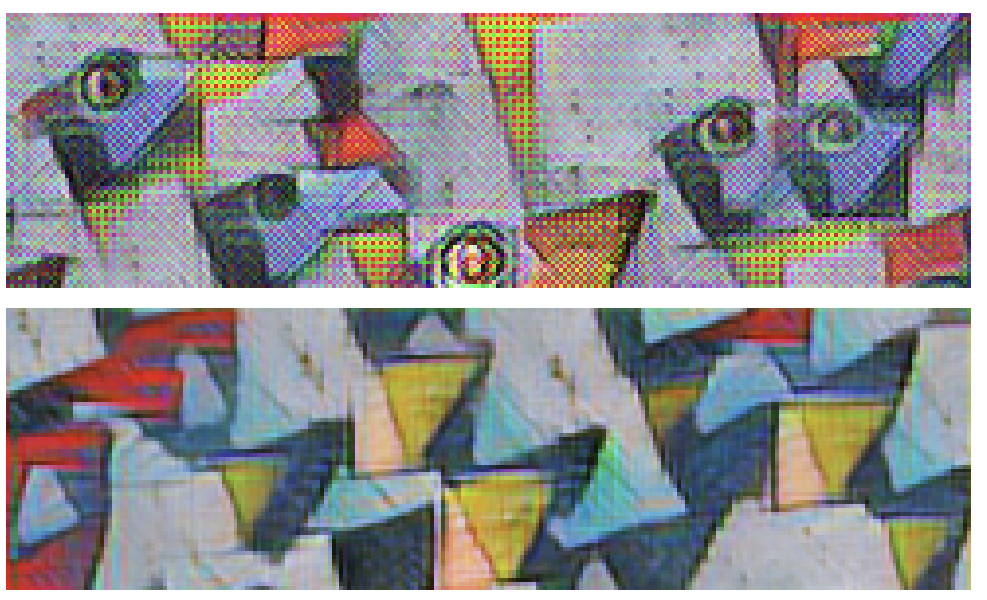
\includegraphics[width=\linewidth]{up_resize}\par\smallskip
    {\footnotesize Em cima: convolução transposta. Embaixo: redimensionar e convoluir.\par}
  \end{minipage}\hfill
  \begin{minipage}[t]{0.48\textwidth}\centering
    {\small\cD{\textbf{Filtro passa-baixa fixo}}}\par\smallskip
    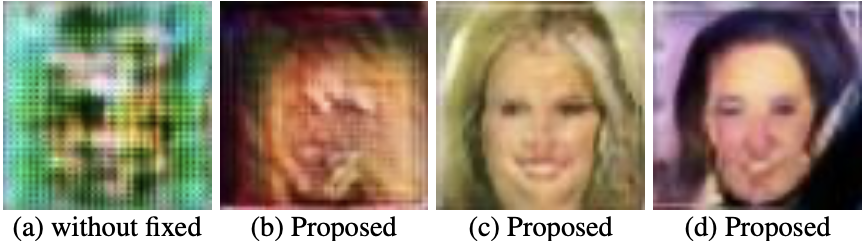
\includegraphics[width=\linewidth]{up_filtro}\par\smallskip
    {\footnotesize (a) sem filtro \textperiodcentered{} (b)--(d) com filtro fixo, cada vez mais suave\par}
  \end{minipage}
  \fonte{Odena, Dumoulin e Olah 2016, Distill \textperiodcentered{} Kinoshita e Kiya 2020, fig. 6 \textperiodcentered{} Karras et al. 2017, 2018 e 2019}
\end{frame}

\section{Problemas da dinâmica adversarial}
\begin{frame}{Roteiro}
  \vspace{4mm}
    {\small\textcolor{coppeGray}{{1. Como uma GAN funciona}}}\par\smallskip
    {\small\textcolor{coppeAccent}{\textbf{2. Problemas na dinâmica adversarial}}}\par\smallskip
    {\footnotesize\textcolor{coppeGray}{Colapso de modos, vanishing gradient, Wasserstein e WGAN-GP}}\par\smallskip
    {\small\textcolor{coppeGray}{{3. Controlar e avaliar}}}\par\smallskip
    {\small\textcolor{coppeGray}{{4. StyleGAN}}}\par\smallskip
    {\small\textcolor{coppeGray}{{5. Pix2Pix e CycleGAN}}}\par\smallskip
    {\small\textcolor{coppeGray}{{6. Aplicações e o nosso exemplo}}}\par\smallskip
\end{frame}

\begin{frame}{Colapso de modos}
  \centering
  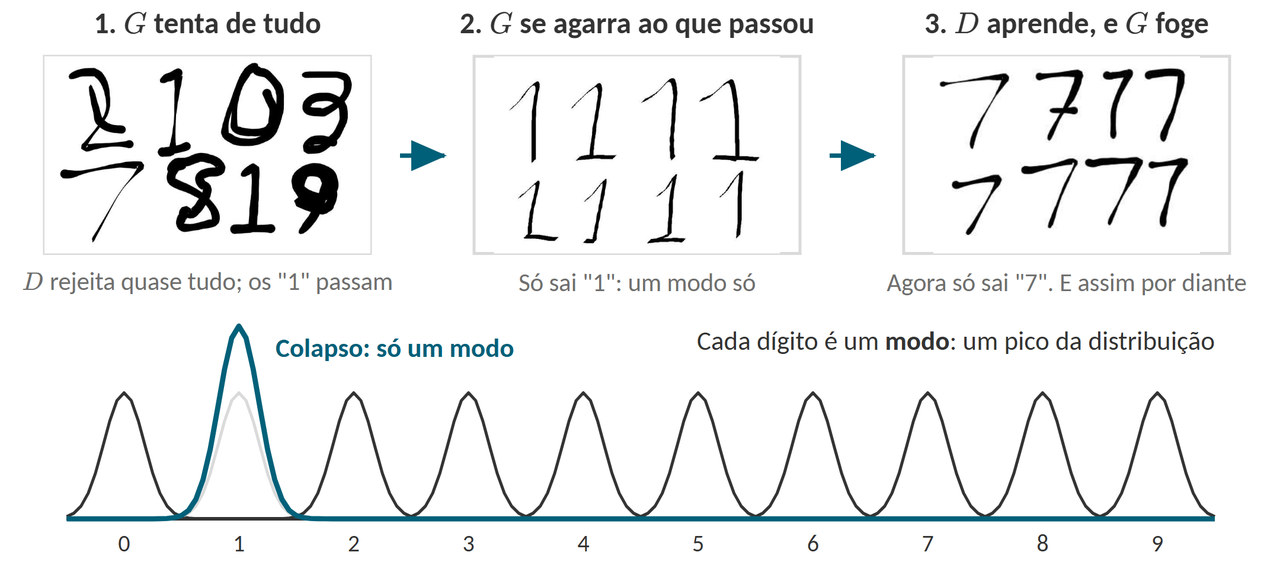
\includegraphics[width=124.4mm]{f_colapso}
  \fonte{Adaptado de DeepLearning.AI C1W3 \textperiodcentered{} ilustração}
\end{frame}

\begin{frame}{Vanishing gradient}
  \centering
  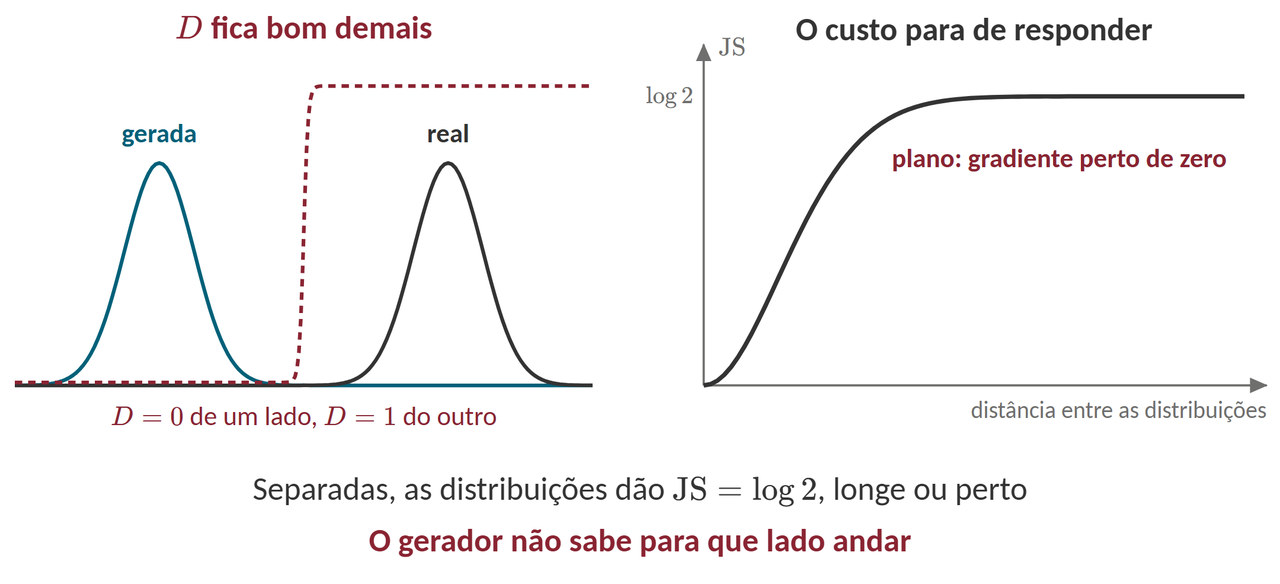
\includegraphics[width=124.4mm]{f_gradiente}
  \fonte{DeepLearning.AI C1W3 \textperiodcentered{} Arjovsky e Bottou 2017 \textperiodcentered{} JS calculada}
\end{frame}

\begin{frame}{Distância de Wasserstein}
  \centering
  \resizebox{53.9mm}{!}{$\displaystyle W(p,q)=\inf_{\gamma\in\Pi(p,q)}\mathbb{E}_{(x,y)\sim\gamma}\Vert x-y\Vert$}\par\vspace{1.5mm}
  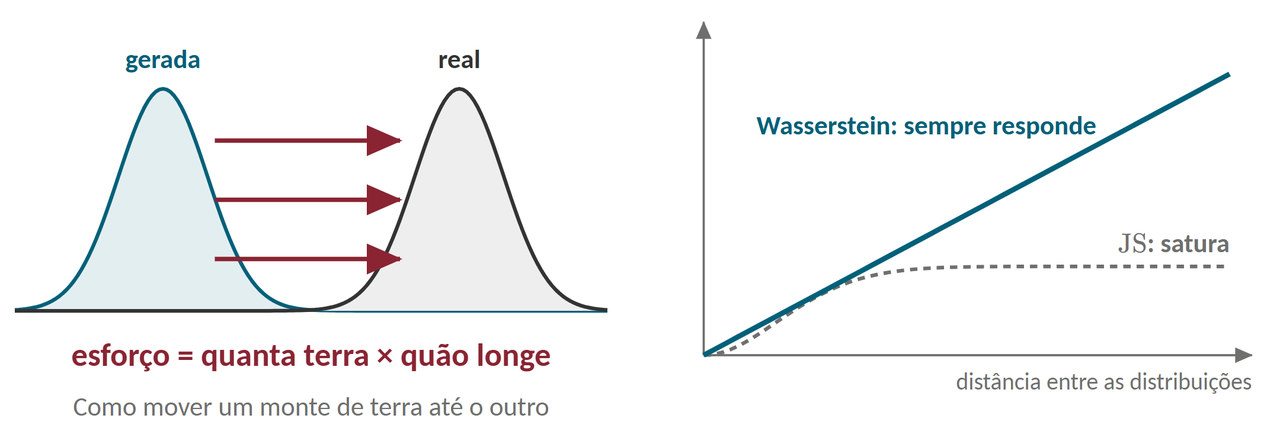
\includegraphics[width=124.4mm]{f_emd}
  \fonte{DeepLearning.AI C1W3 \textperiodcentered{} Arjovsky et al. 2017, eq. 1}
\end{frame}

\begin{frame}{WGAN: de discriminador a crítico}
  \centering
  \resizebox{74.4mm}{!}{$\displaystyle \text{BCE:}\quad\min_G\max_D\ \mathbb{E}\log D(x)+\mathbb{E}\log\big(1-D(G(z))\big)$}\par\vspace{1.5mm}
  \resizebox{58.0mm}{!}{$\displaystyle \text{W-loss:}\quad\min_G\max_C\ \mathbb{E}\,C(x)-\mathbb{E}\,C(G(z))$}\par\vspace{1.5mm}
  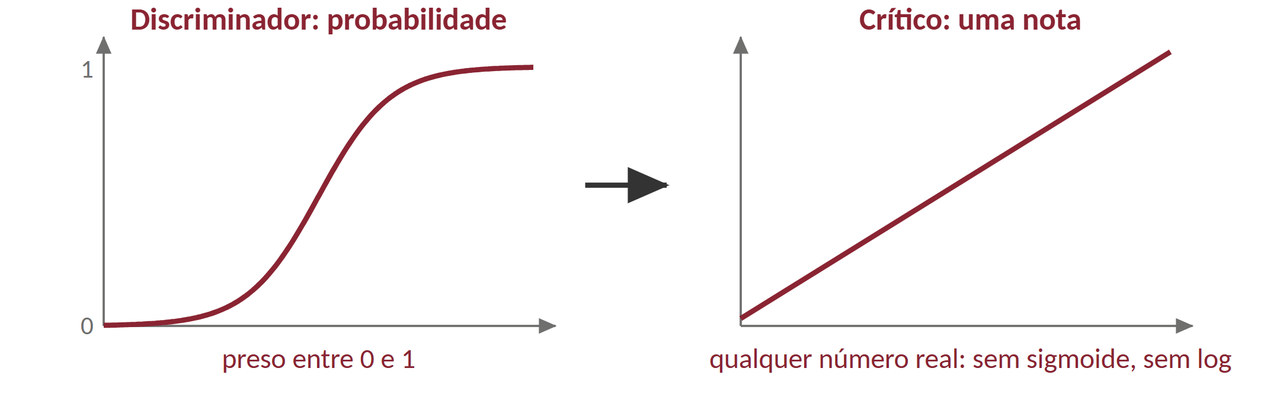
\includegraphics[width=124.4mm]{f_wloss}
  \fonte{DeepLearning.AI C1W3 \textperiodcentered{} Arjovsky et al. 2017, eq. 3}
\end{frame}

\begin{frame}{WGAN: crítico 1-Lipschitz}
  \centering
  \resizebox{60.3mm}{!}{$\displaystyle W(p,q)=\sup_{\Vert C\Vert_L\le 1}\ \mathbb{E}_{x\sim p}C(x)-\mathbb{E}_{x\sim q}C(x)$}\par\vspace{1.5mm}
  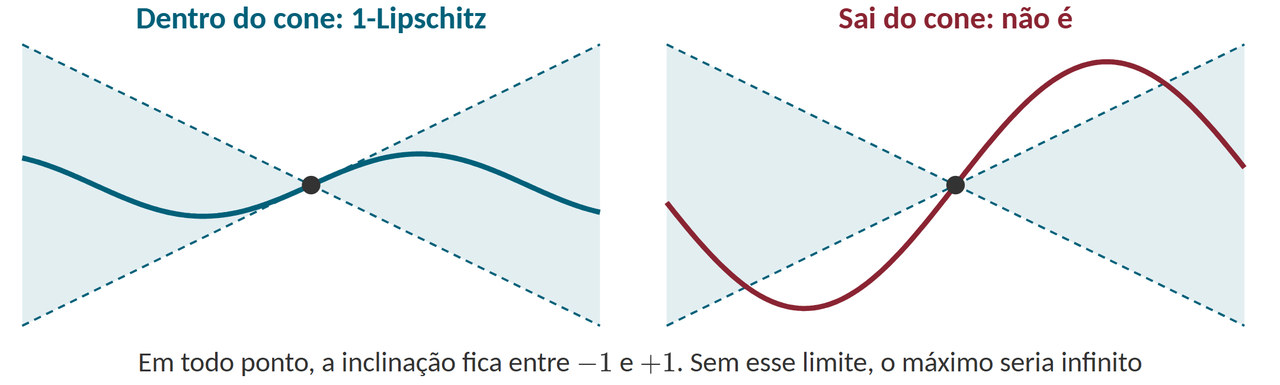
\includegraphics[width=124.4mm]{f_lip}
  \fonte{DeepLearning.AI C1W3 \textperiodcentered{} Arjovsky et al. 2017, eq. 2}
\end{frame}



\begin{frame}{WGAN-GP: penalidade de gradiente}
  \centering
  \resizebox{112.5mm}{!}{$\displaystyle \min_G\max_C\ \underbrace{\mathbb{E}\,C(x)-\mathbb{E}\,C(G(z))}_{\text{W-loss}}-\lambda\,\underbrace{\mathbb{E}\big(\Vert\nabla_{\hat x}C(\hat x)\Vert_2-1\big)^2}_{\text{penalidade de gradiente}},\qquad \hat x=\epsilon x+(1-\epsilon)G(z)$}\par\vspace{1.5mm}
  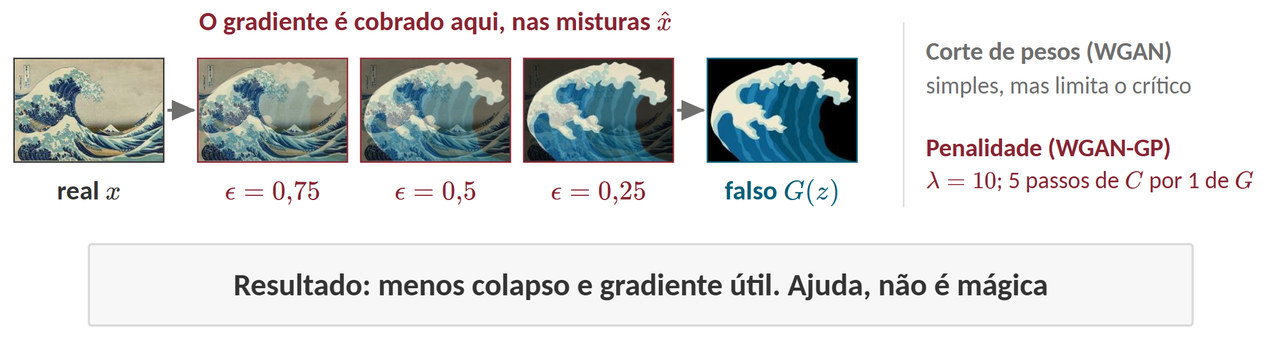
\includegraphics[width=124.4mm]{f_gp}
  \fonte{Gulrajani et al. 2017, eq. 3 \textperiodcentered{} DeepLearning.AI C1W3 \textperiodcentered{}}
\end{frame}

\begin{frame}{WGAN contra o vanishing gradient}
  \centering
  \resizebox{78.0mm}{!}{$\displaystyle \nabla_{\theta_g}\,\text{custo}\big(G(z)\big)=\underbrace{\nabla_x\,\text{custo}(x)\big|_{x=G(z)}}_{\text{é aqui que o sinal vive ou morre}}\ \cdot\ \underbrace{\frac{\partial G(z)}{\partial\theta_g}}_{\text{a rede do gerador}}$}\par\vspace{1.5mm}
  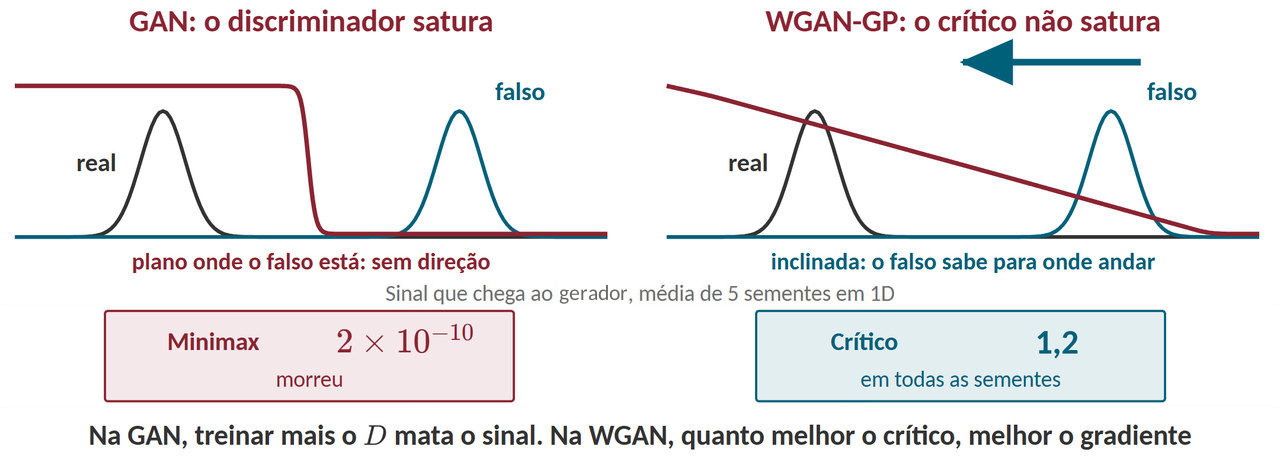
\includegraphics[width=124.4mm]{f_wgrad}
  \fonte{Arjovsky et al. 2017, fig. 2 e seção 3 \textperiodcentered{} Arjovsky e Bottou 2017, teo. 2.4 e 2.6 \textperiodcentered{} medida nossa: exemplos/critico\_1d.py}
\end{frame}

\section{Controlar e avaliar}
\begin{frame}{Roteiro}
  \vspace{4mm}
    {\small\textcolor{coppeGray}{{1. Como uma GAN funciona}}}\par\smallskip
    {\small\textcolor{coppeGray}{{2. Problemas na dinâmica adversarial}}}\par\smallskip
    {\small\textcolor{coppeAccent}{\textbf{3. Controlar e avaliar}}}\par\smallskip
    {\footnotesize\textcolor{coppeGray}{Condicionar, andar em z e medir com a FID}}\par\smallskip
    {\small\textcolor{coppeGray}{{4. StyleGAN}}}\par\smallskip
    {\small\textcolor{coppeGray}{{5. Pix2Pix e CycleGAN}}}\par\smallskip
    {\small\textcolor{coppeGray}{{6. Aplicações e o nosso exemplo}}}\par\smallskip
\end{frame}

\begin{frame}{GAN condicional}
  \centering
  \resizebox{76.2mm}{!}{$\displaystyle \min_G\max_D\ \mathbb{E}\log D(x\mid y)+\mathbb{E}\log\big(1-D(G(z\mid y)\mid y)\big)$}\par\vspace{1.5mm}
  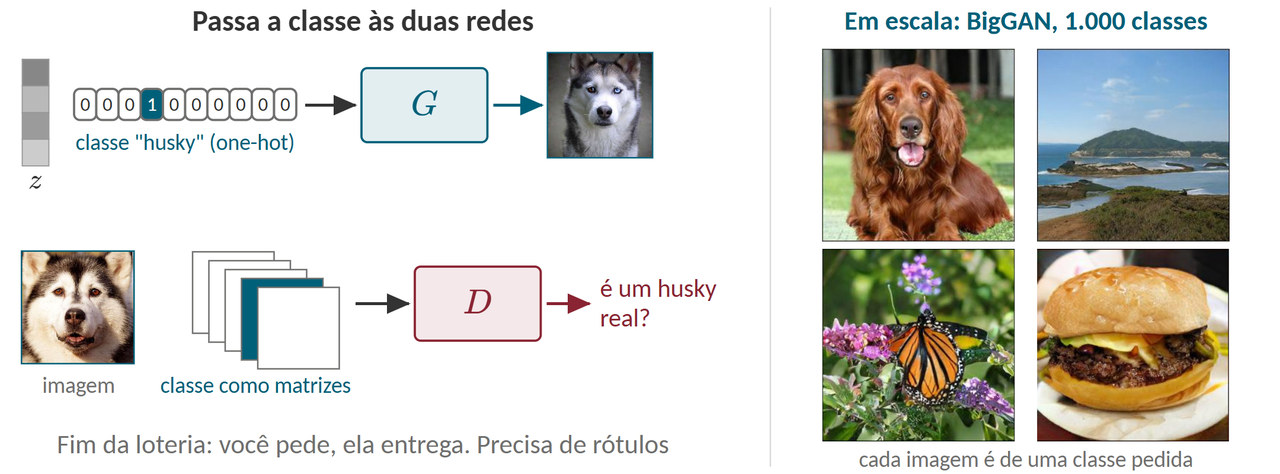
\includegraphics[width=124.4mm]{f_cond}
  \fonte{Mirza e Osindero 2014 \textperiodcentered{} DeepLearning.AI C1W4 \textperiodcentered{} BigGAN, Brock et al. 2018, fig. 1}
\end{frame}

\begin{frame}{Controlar: andar no espaço z}
  \centering
  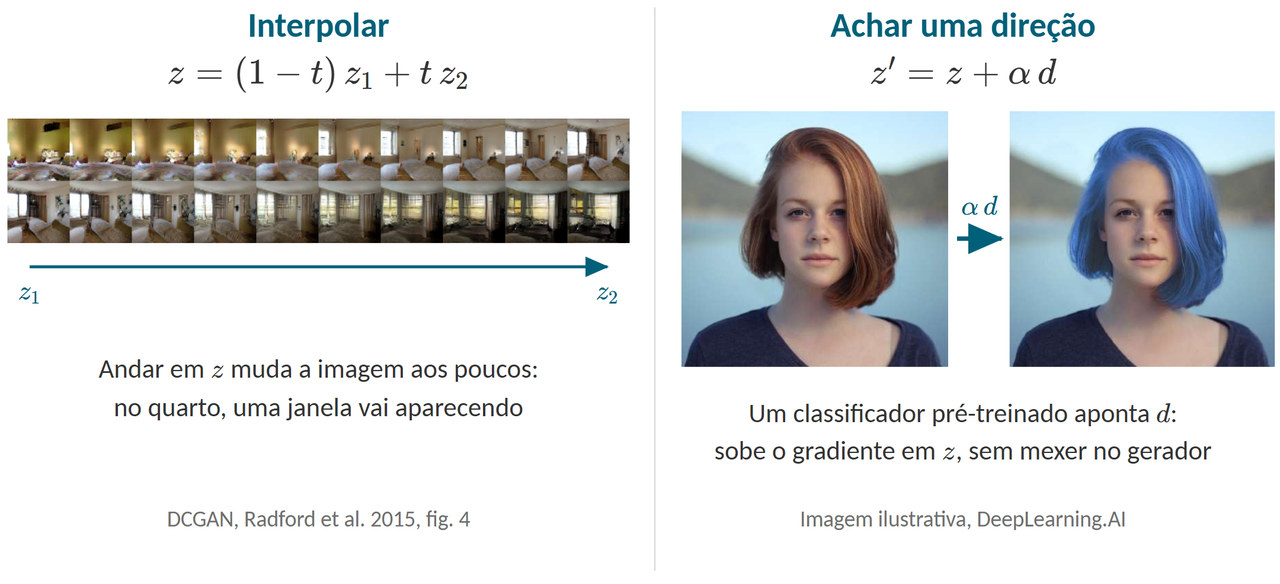
\includegraphics[width=124.4mm]{f_espz}
  \fonte{Radford et al. 2015, fig. 4 \textperiodcentered{} DeepLearning.AI C1W4}
\end{frame}

\begin{frame}{O problema: z emaranhado}
  \centering
  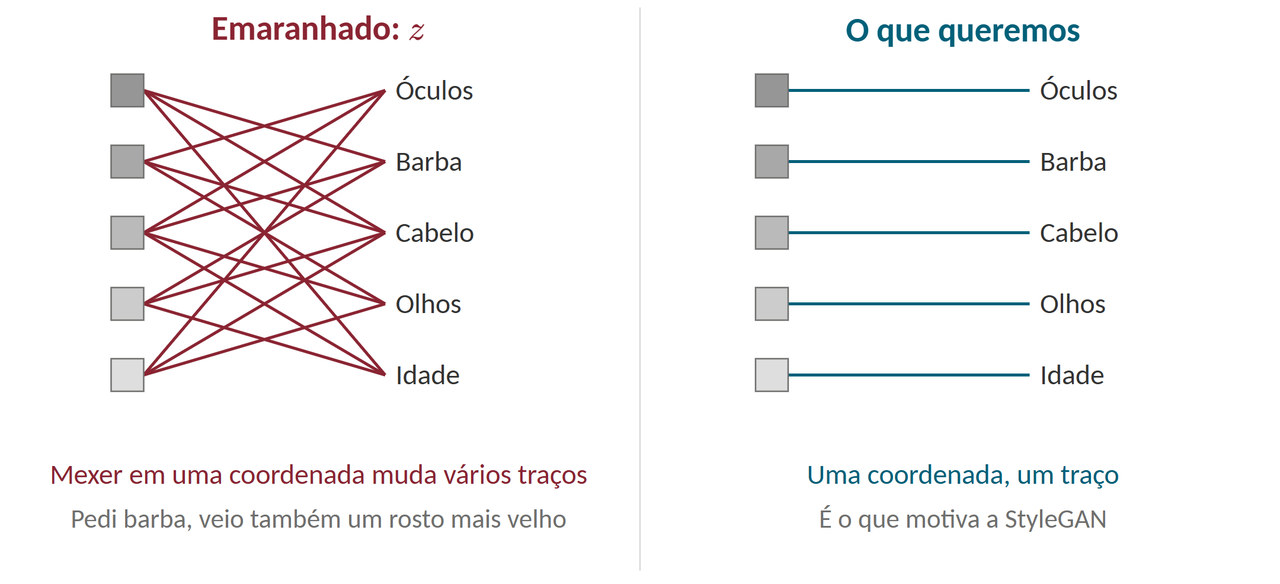
\includegraphics[width=124.4mm]{f_emaranhado}
  \fonte{Adaptado de DeepLearning.AI C1W4 \textperiodcentered{} esquema}
\end{frame}

\begin{frame}{Como avaliar sem gabarito?}
  \centering
  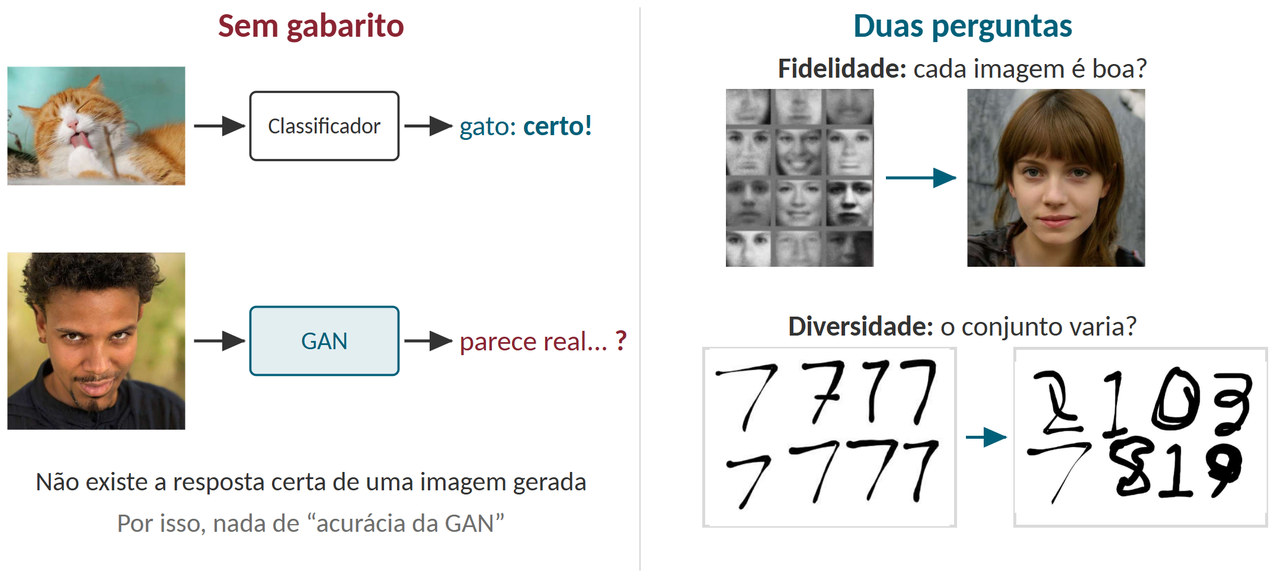
\includegraphics[width=124.4mm]{f_avaliar}
  \fonte{Adaptado de DeepLearning.AI C2W1 \textperiodcentered{} Goodfellow seção 20.14}
\end{frame}

\begin{frame}{FID}
  \centering
  \resizebox{73.2mm}{!}{$\displaystyle \mathrm{FID}=\underbrace{\Vert\mu_r-\mu_g\Vert_2^2}_{\text{no mesmo lugar?}}+\underbrace{\mathrm{Tr}\big(\Sigma_r+\Sigma_g-2(\Sigma_r\Sigma_g)^{1/2}\big)}_{\text{com a mesma forma?}}$}\par\vspace{1.5mm}
  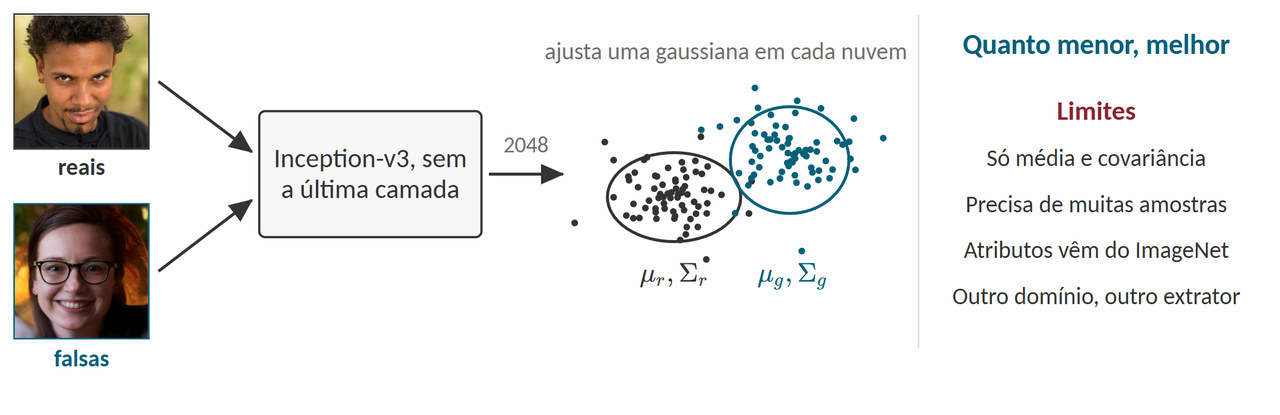
\includegraphics[width=124.4mm]{f_fid}
  \fonte{Heusel et al. 2017, eq. 6 \textperiodcentered{} DeepLearning.AI C2W1}
\end{frame}

\begin{frame}{Precisão, revocação e truncamento}
  \centering
  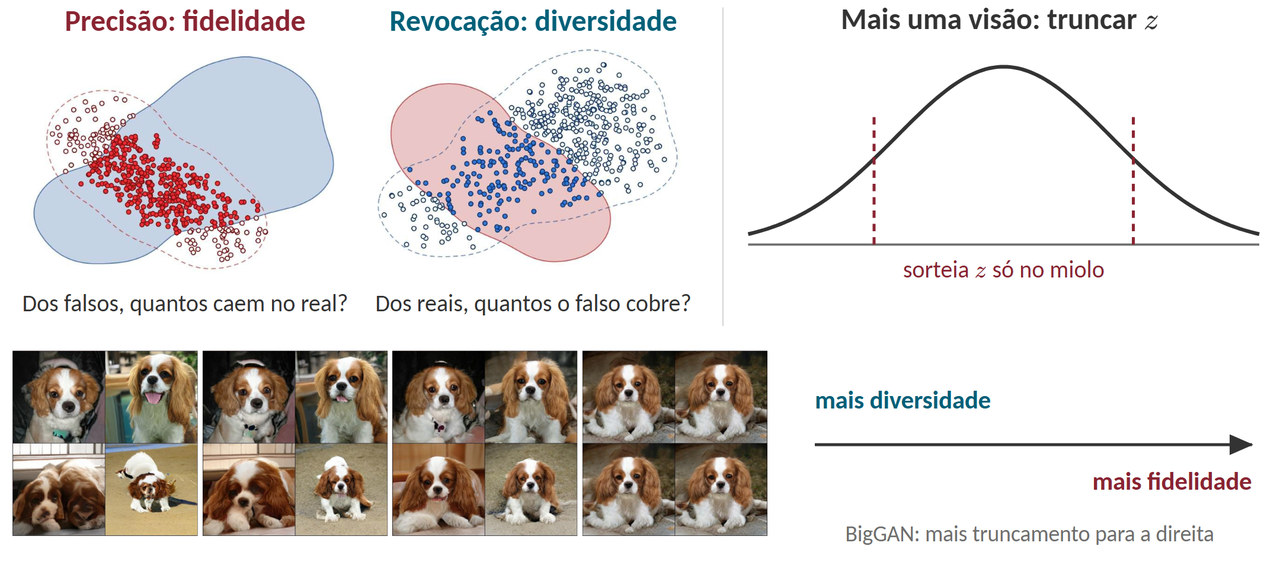
\includegraphics[width=124.4mm]{f_pr}
  \fonte{Kynkäänniemi et al. 2019 \textperiodcentered{} BigGAN, Brock et al. 2018 \textperiodcentered{} DeepLearning.AI C2W1}
\end{frame}

\section{StyleGAN}
\begin{frame}{Roteiro}
  \vspace{4mm}
    {\small\textcolor{coppeGray}{{1. Como uma GAN funciona}}}\par\smallskip
    {\small\textcolor{coppeGray}{{2. Problemas na dinâmica adversarial}}}\par\smallskip
    {\small\textcolor{coppeGray}{{3. Controlar e avaliar}}}\par\smallskip
    {\small\textcolor{coppeAccent}{\textbf{4. StyleGAN}}}\par\smallskip
    {\footnotesize\textcolor{coppeGray}{Crescimento progressivo, mapeamento, AdaIN, mistura e ruído}}\par\smallskip
    {\small\textcolor{coppeGray}{{5. Pix2Pix e CycleGAN}}}\par\smallskip
    {\small\textcolor{coppeGray}{{6. Aplicações e o nosso exemplo}}}\par\smallskip
\end{frame}

\begin{frame}{StyleGAN: as metas}
  \centering
  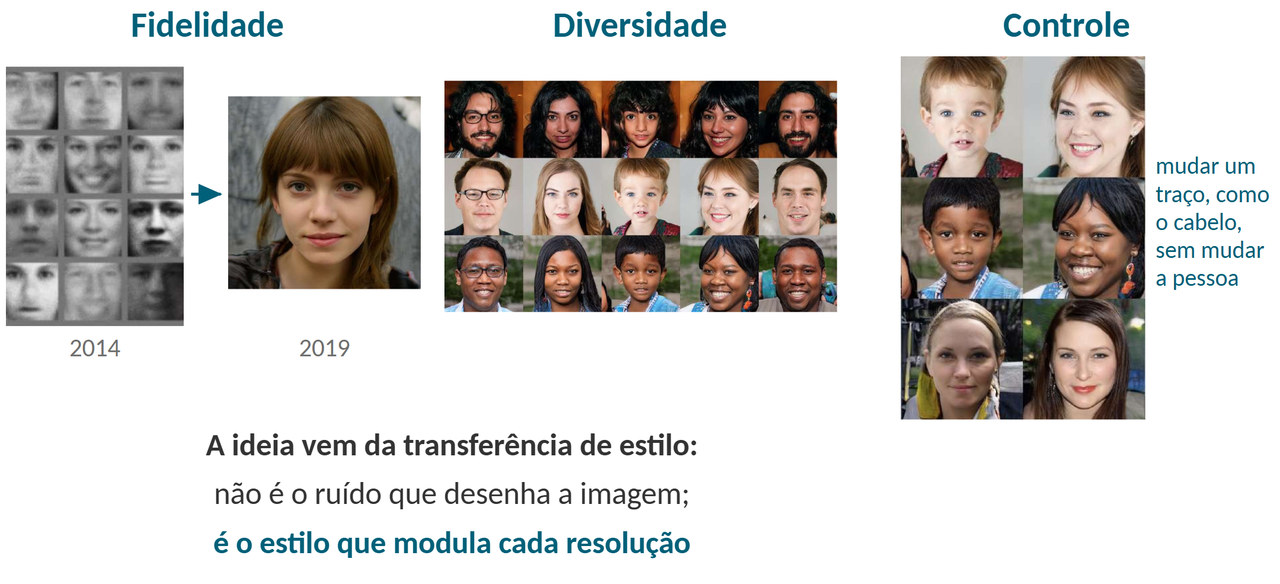
\includegraphics[width=124.4mm]{f_style_meta}
  \fonte{Karras et al. 2018 \textperiodcentered{} DeepLearning.AI C2W3}
\end{frame}

\begin{frame}{O gerador baseado em estilo}
  \centering
  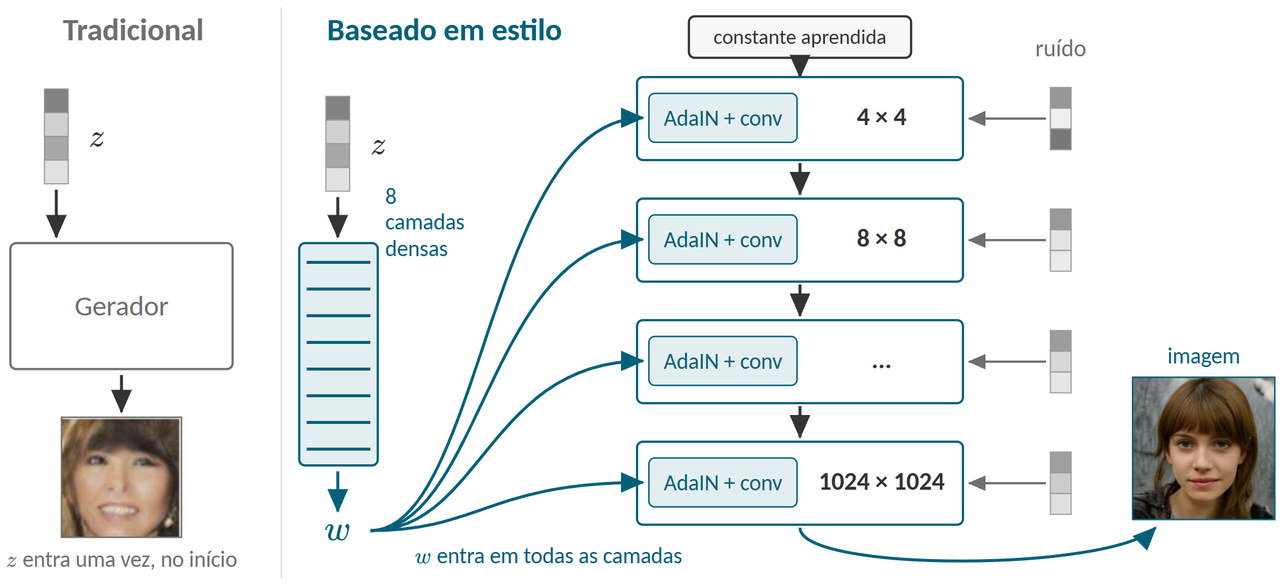
\includegraphics[width=124.4mm]{f_style_arq}
  \fonte{Redesenhado de Karras et al. 2018, fig. 1, e DeepLearning.AI C2W3}
\end{frame}

\begin{frame}{Peça 1: crescimento progressivo}
  \centering
  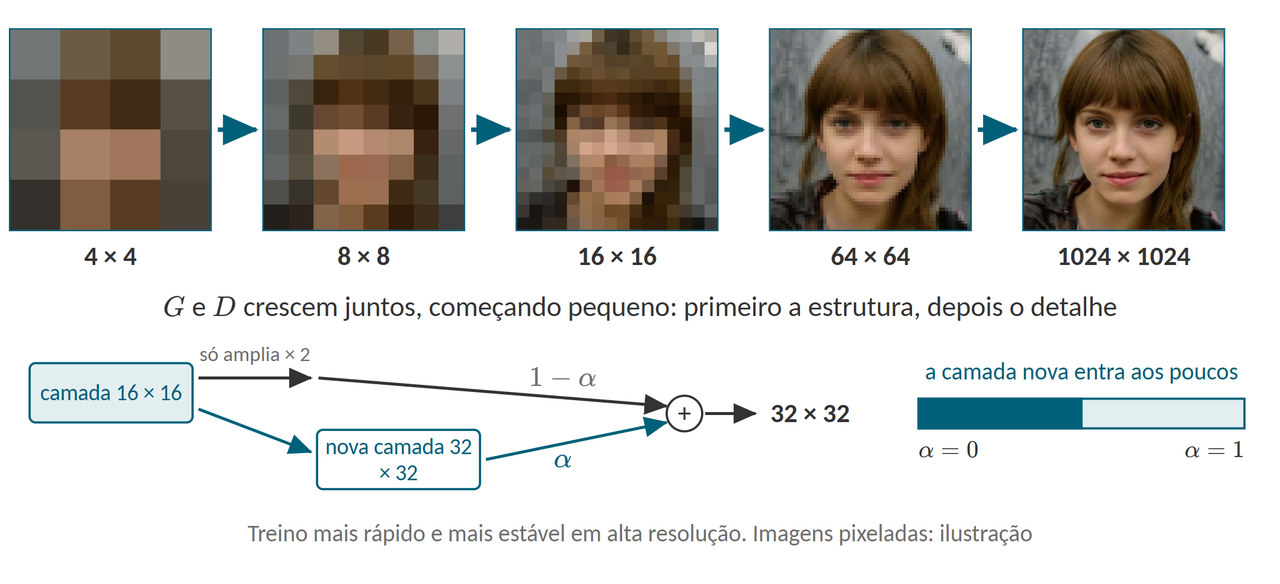
\includegraphics[width=124.4mm]{f_prog}
  \fonte{Karras et al. 2017, fig. 2 \textperiodcentered{} DeepLearning.AI C2W3}
\end{frame}

\begin{frame}{Peça 2: rede de mapeamento}
  \centering
  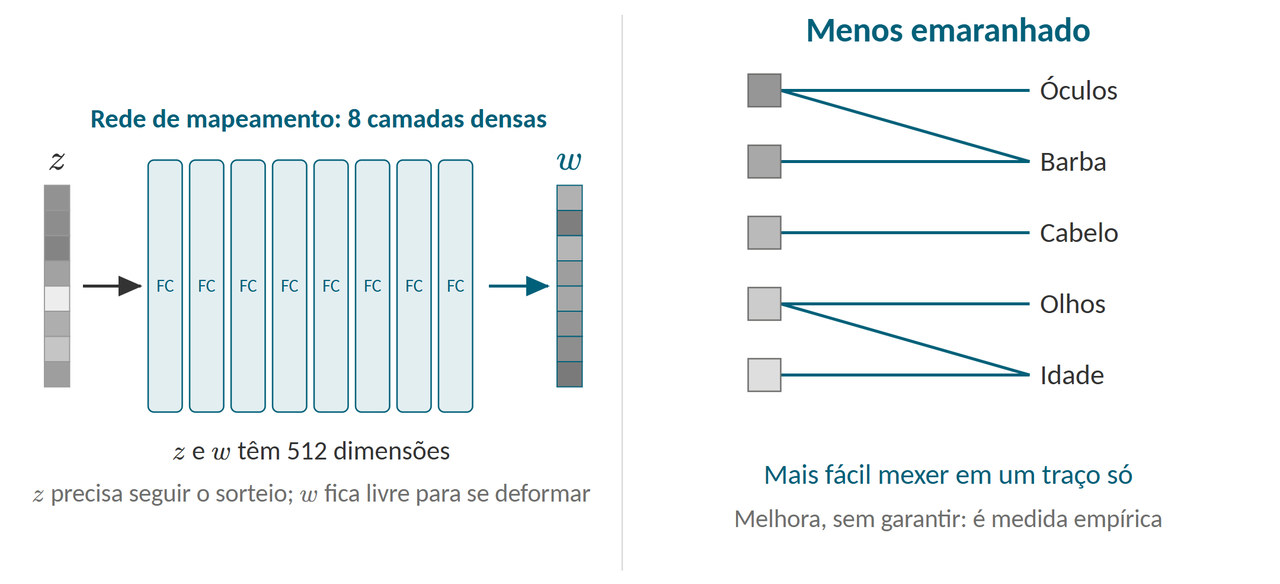
\includegraphics[width=124.4mm]{f_map}
  \fonte{Karras et al. 2018 \textperiodcentered{} adaptado de DeepLearning.AI C2W3}
\end{frame}

\begin{frame}{Peça 3: AdaIN}
  \centering
  \resizebox{73.3mm}{!}{$\displaystyle \mathrm{AdaIN}(x_i,y)=\underbrace{y_{s,i}}_{\text{novo desvio}}\ \underbrace{\frac{x_i-\mu(x_i)}{\sigma(x_i)}}_{\text{tira o estilo antigo}}+\underbrace{y_{b,i}}_{\text{nova média}}$}\par\vspace{1.5mm}
  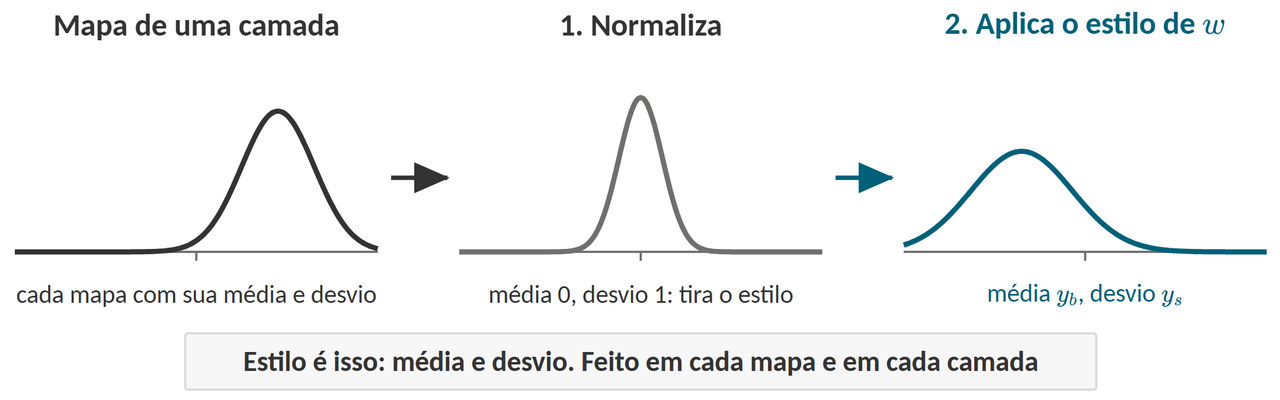
\includegraphics[width=124.4mm]{f_adain}
  \fonte{Karras et al. 2018, eq. 1 \textperiodcentered{} DeepLearning.AI C2W3}
\end{frame}

\begin{frame}{Peça 4: mistura de estilos}
  \begin{minipage}[t]{0.47\textwidth}\vspace{0pt}\centering
    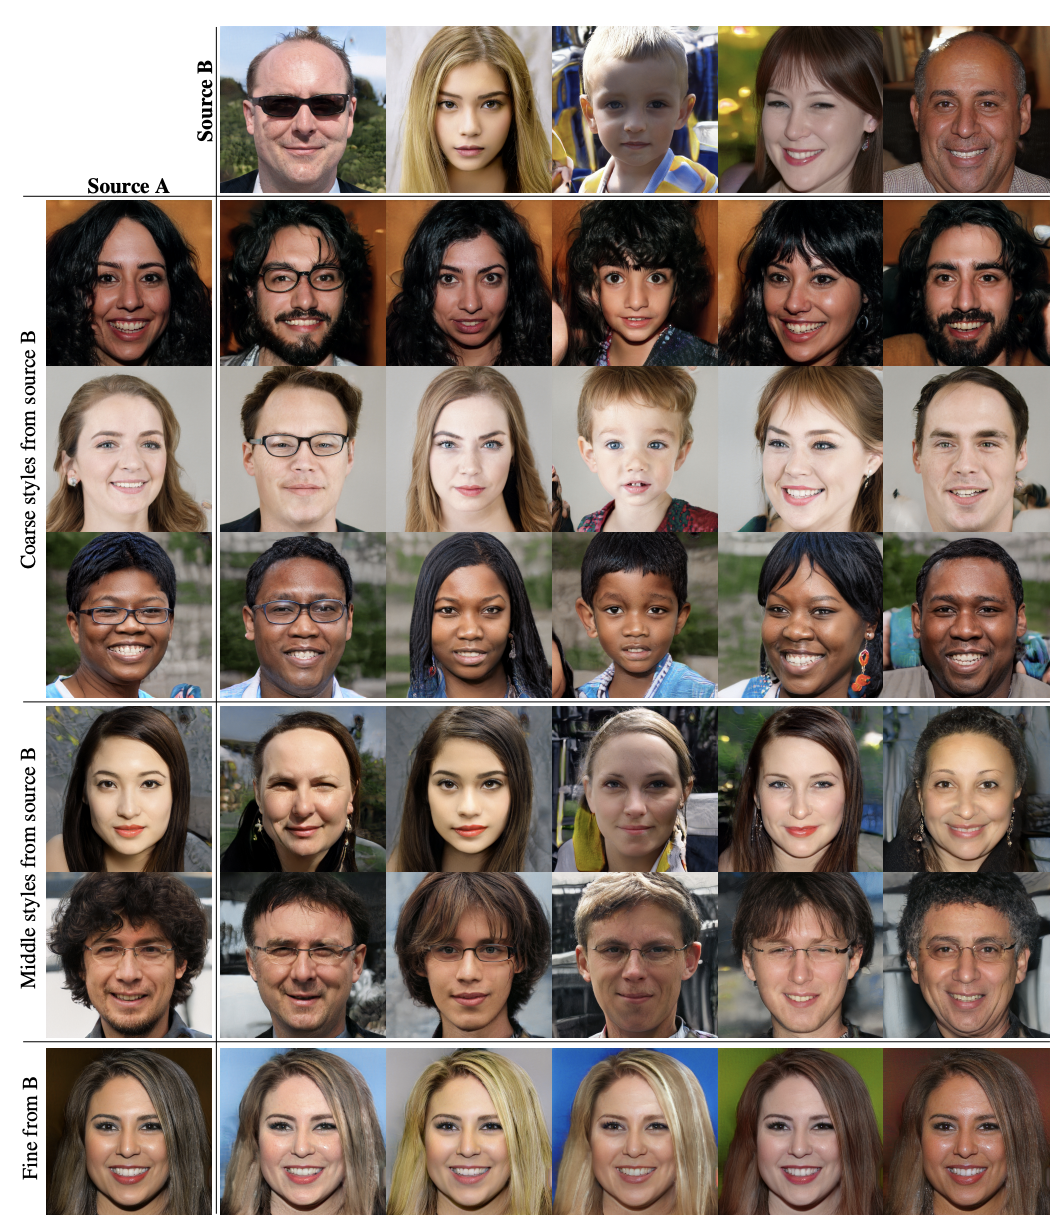
\includegraphics[height=64mm]{f_mistura_completa}
  \end{minipage}\hfill
  \begin{minipage}[t]{0.5\textwidth}\vspace{0pt}
    \vspace{10.2mm}% altura da linha da fonte B
    \bloco{coppeAccent}{26.2mm}{Grosso de B}{$4^2$ a $8^2$: pose, formato do rosto, óculos}
    \bloco{coppeGraphite}{17.6mm}{Médio de B}{$16^2$ a $32^2$: traços do rosto, penteado, olhos}
    \bloco{coppeWine}{9.2mm}{Fino de B}{$64^2$ a $1024^2$: cores e microestrutura}
  \end{minipage}
  \fonte{Karras et al. 2018, fig. 3}
\end{frame}

\begin{frame}{Peça 5: ruído estocástico}
  \centering
  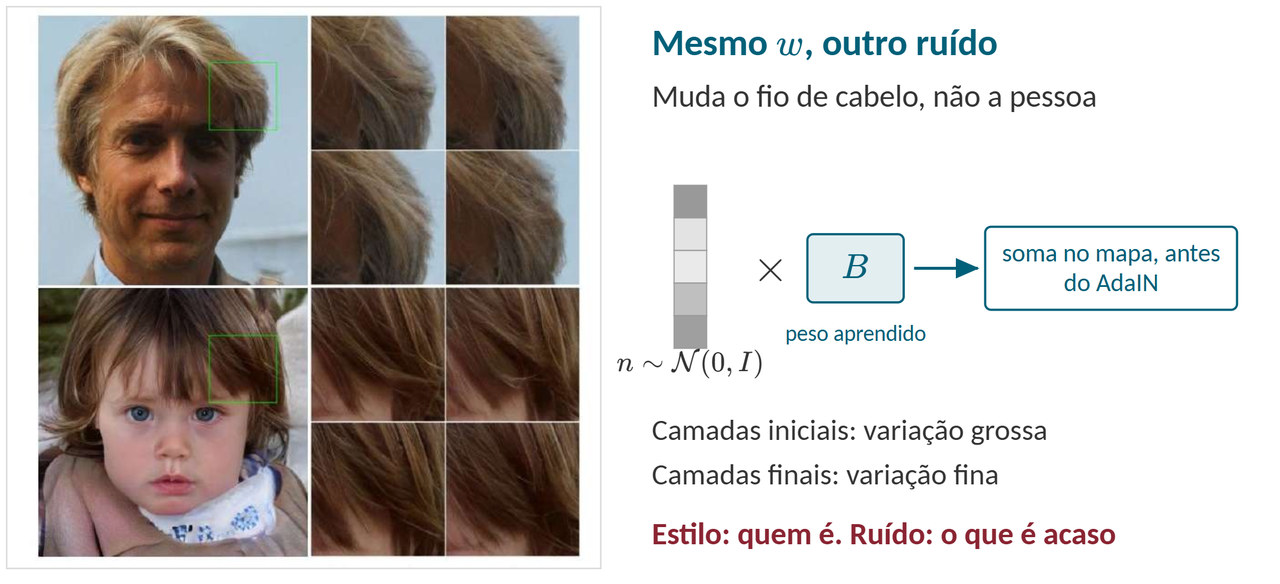
\includegraphics[width=124.4mm]{f_ruido}
  \fonte{Karras et al. 2018, fig. 4, em DeepLearning.AI C2W3}
\end{frame}


\section{Pix2Pix e CycleGAN}
\begin{frame}{Roteiro}
  \vspace{4mm}
    {\small\textcolor{coppeGray}{{1. Como uma GAN funciona}}}\par\smallskip
    {\small\textcolor{coppeGray}{{2. Problemas na dinâmica adversarial}}}\par\smallskip
    {\small\textcolor{coppeGray}{{3. Controlar e avaliar}}}\par\smallskip
    {\small\textcolor{coppeGray}{{4. StyleGAN}}}\par\smallskip
    {\small\textcolor{coppeAccent}{\textbf{5. Pix2Pix e CycleGAN}}}\par\smallskip
    {\footnotesize\textcolor{coppeGray}{Traduzir imagens, com pares e sem pares}}\par\smallskip
    {\small\textcolor{coppeGray}{{6. Aplicações e o nosso exemplo}}}\par\smallskip
\end{frame}

\begin{frame}{Tradução de imagem para imagem}
  \centering
  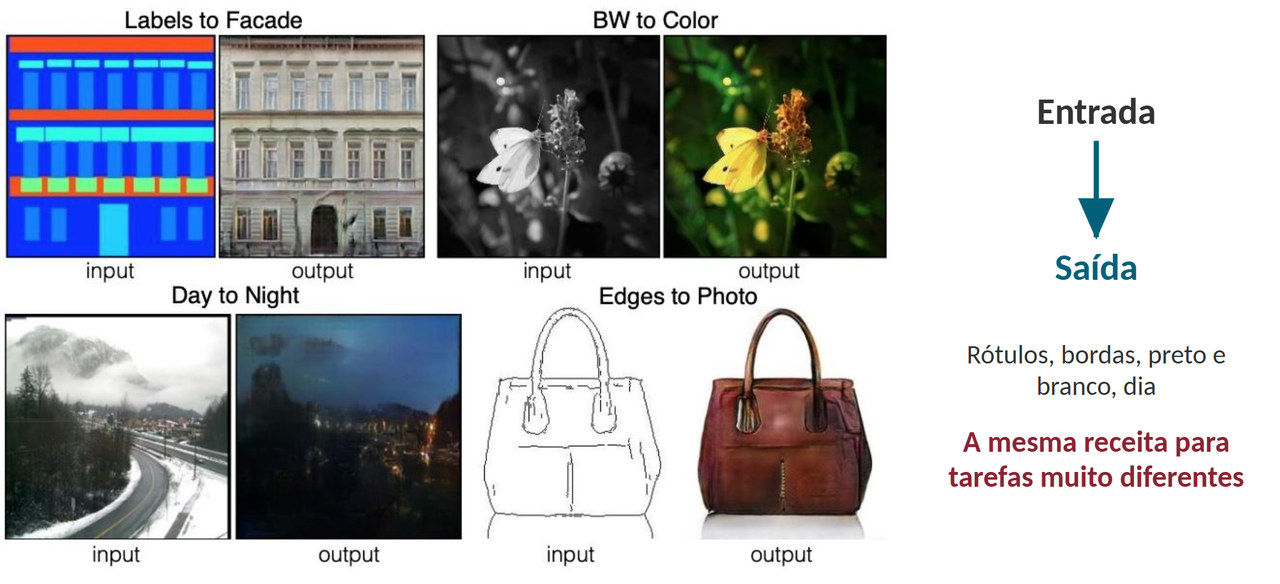
\includegraphics[width=124.4mm]{f_traducao}
  \fonte{Isola et al. 2016, fig. 1, em DeepLearning.AI C3W2}
\end{frame}

\begin{frame}{Pix2Pix}
  \centering
  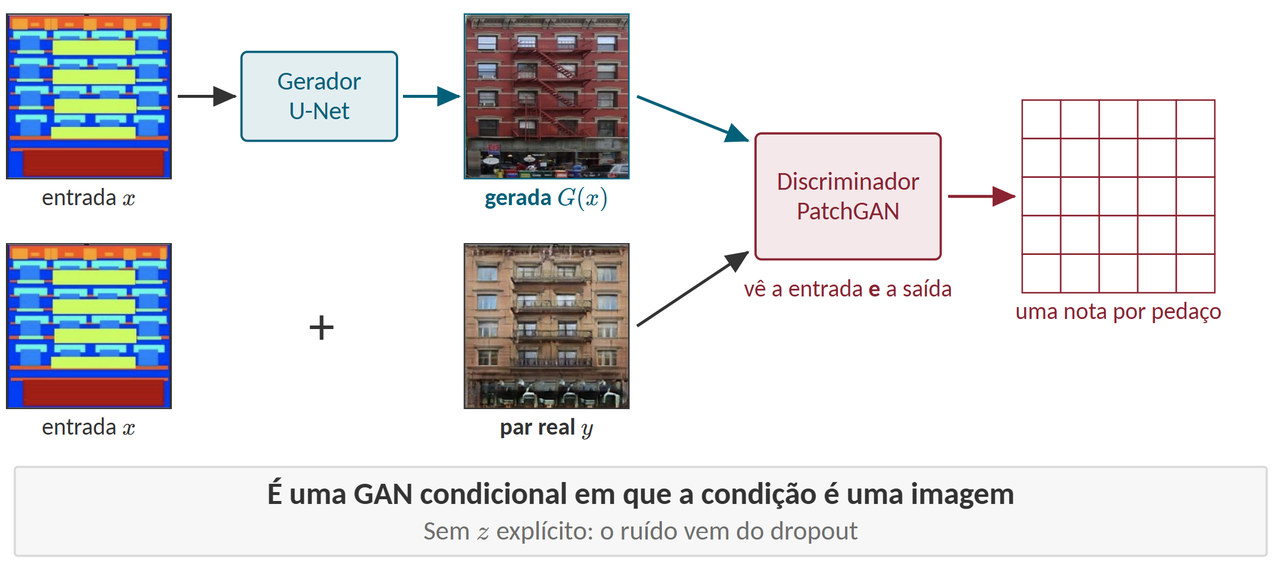
\includegraphics[width=124.4mm]{f_pix2pix}
  \fonte{Isola et al. 2016 \textperiodcentered{} adaptado de DeepLearning.AI C3W2}
\end{frame}

\begin{frame}{Pix2Pix: gerador U-Net}
  \centering
  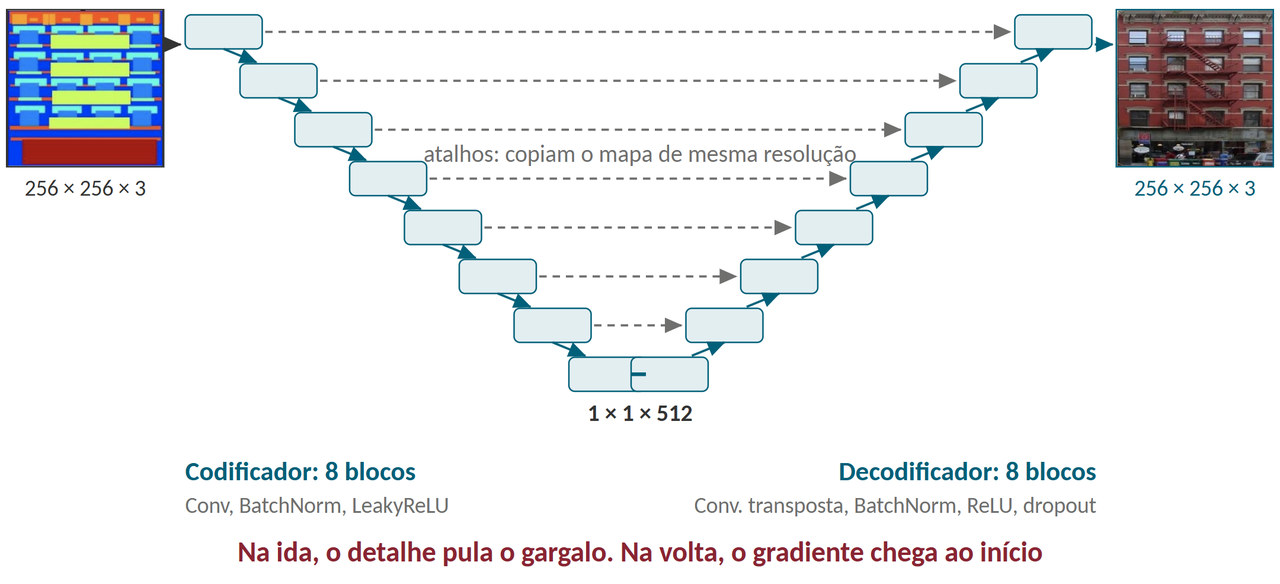
\includegraphics[width=124.4mm]{f_unet}
  \fonte{Isola et al. 2016 \textperiodcentered{} adaptado de DeepLearning.AI C3W2}
\end{frame}

\begin{frame}{Pix2Pix: PatchGAN e o custo}
  \centering
  \resizebox{93.5mm}{!}{$\displaystyle G^{*}=\arg\min_G\max_D\ \underbrace{\mathcal{L}_{\text{cGAN}}(G,D)}_{\text{parece real?}}+\lambda\,\underbrace{\mathbb{E}\,\Vert y-G(x)\Vert_1}_{\text{parece o par certo?}},\qquad \lambda=100$}\par\vspace{1.5mm}
  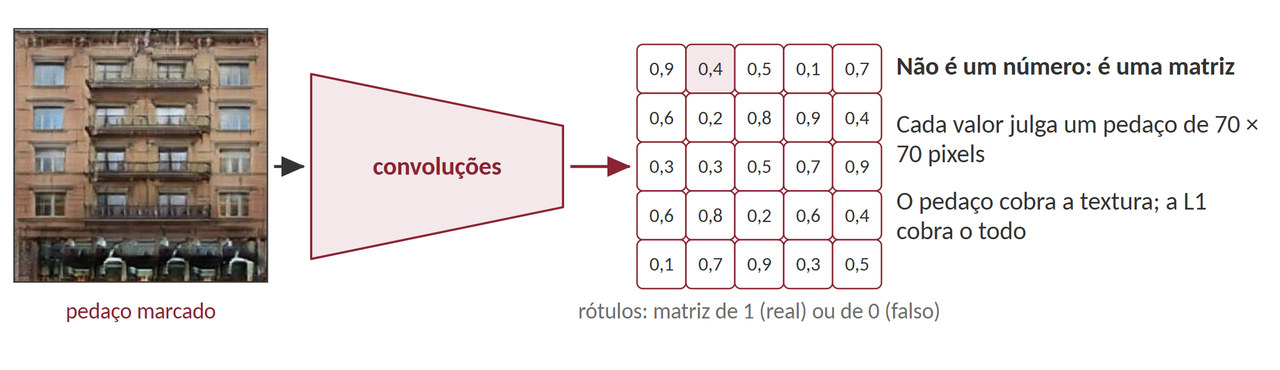
\includegraphics[width=124.4mm]{f_patchgan}
  \fonte{Isola et al. 2016, eq. 4 \textperiodcentered{} adaptado de DeepLearning.AI C3W2}
\end{frame}

\begin{frame}{Os sucessores do Pix2Pix}
  \centering
  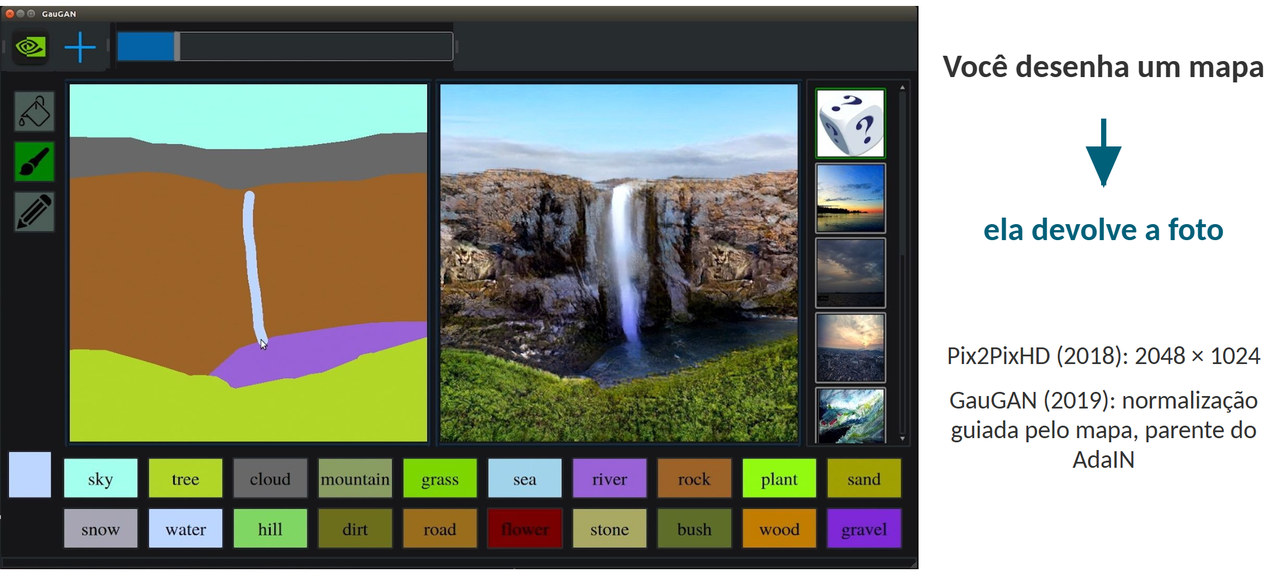
\includegraphics[width=124.4mm]{f_gaugan}
  \fonte{GauGAN, Park et al. 2019, em DeepLearning.AI C3W2 \textperiodcentered{} Pix2PixHD, Wang et al. 2017}
\end{frame}

\begin{frame}{E quando não há pares?}
  \centering
  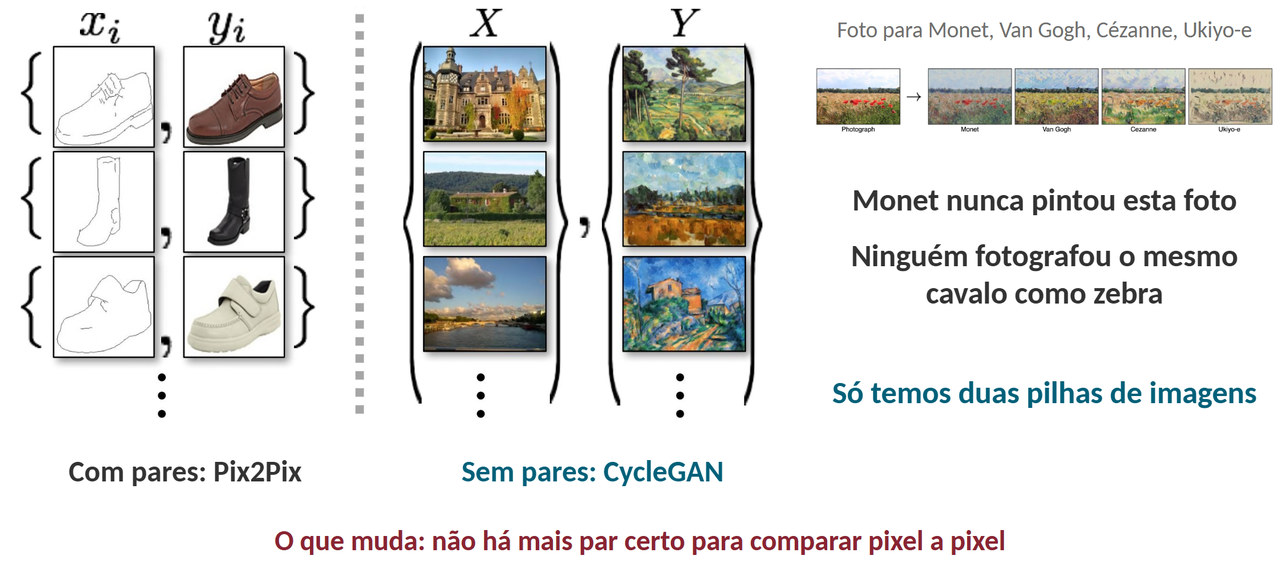
\includegraphics[width=124.4mm]{f_pares}
  \fonte{Zhu et al. 2017, fig. 1 e 2, em DeepLearning.AI C3W3}
\end{frame}

\begin{frame}{CycleGAN: o ciclo}
  \centering
  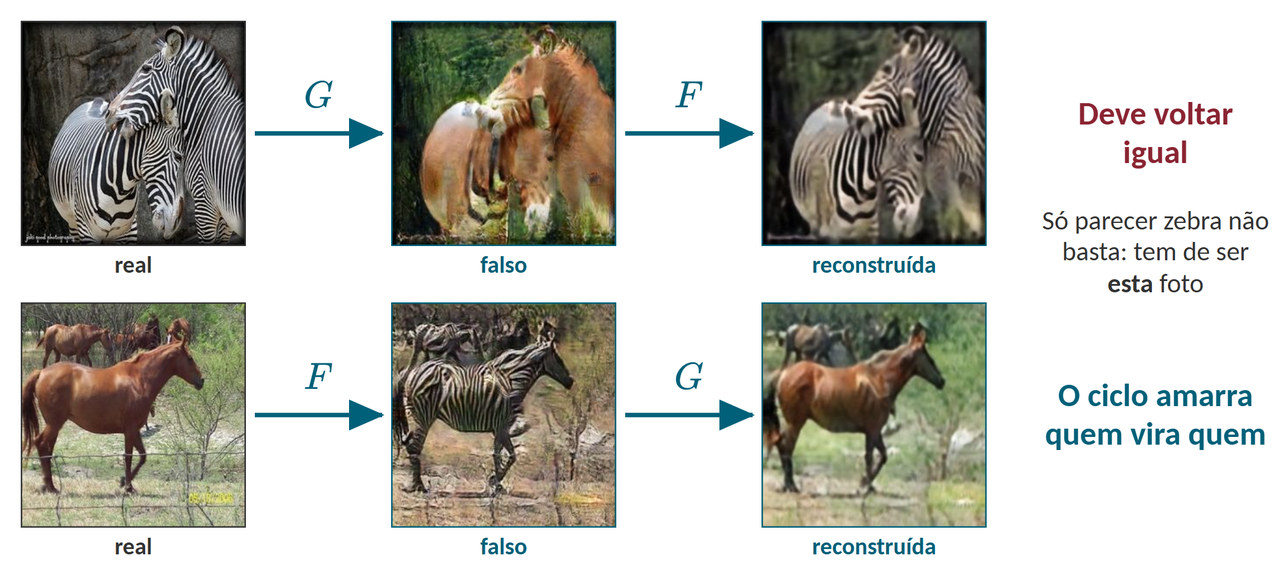
\includegraphics[width=124.4mm]{f_ciclo}
  \fonte{Zhu et al. 2017 \textperiodcentered{} imagens: DeepLearning.AI C3W3 (togheppi/CycleGAN)}
\end{frame}

\begin{frame}{CycleGAN: dois GANs, quatro redes}
  \centering
  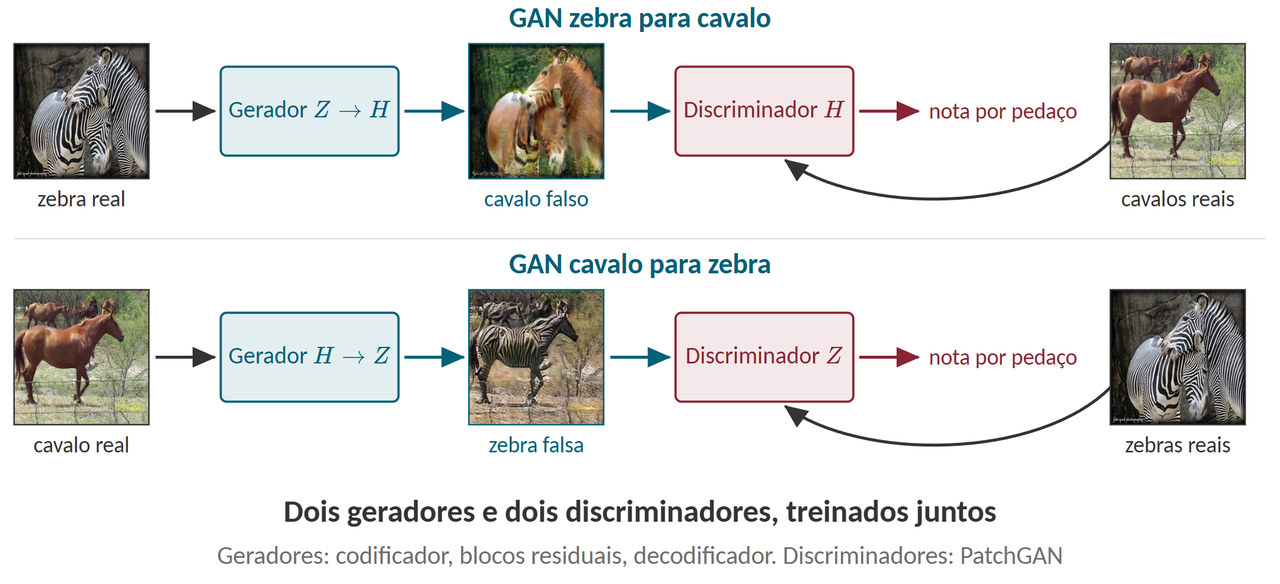
\includegraphics[width=124.4mm]{f_dois}
  \fonte{Zhu et al. 2017 \textperiodcentered{} adaptado de DeepLearning.AI C3W3}
\end{frame}

\begin{frame}{CycleGAN: o custo}
  \centering
  \resizebox{74.4mm}{!}{$\displaystyle \mathcal{L}=\underbrace{\mathcal{L}_{\text{GAN}}(G,D_Y)+\mathcal{L}_{\text{GAN}}(F,D_X)}_{\text{parecer do outro domínio}}+\lambda\,\underbrace{\mathcal{L}_{\text{cyc}}(G,F)}_{\text{voltar ao original}}$}\par\vspace{1.5mm}
  \resizebox{77.6mm}{!}{$\displaystyle \mathcal{L}_{\text{cyc}}(G,F)=\mathbb{E}_x\Vert F(G(x))-x\Vert_1+\mathbb{E}_y\Vert G(F(y))-y\Vert_1$}\par\vspace{1.5mm}
  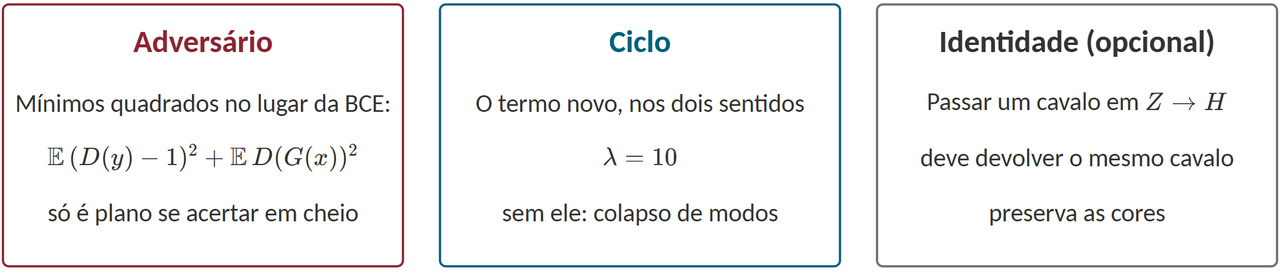
\includegraphics[width=124.4mm]{f_ciclo_custo}
  \fonte{Zhu et al. 2017, eq. 2 e 3 \textperiodcentered{} DeepLearning.AI C3W3}
\end{frame}

\begin{frame}{CycleGAN: cada termo importa}
  \centering
  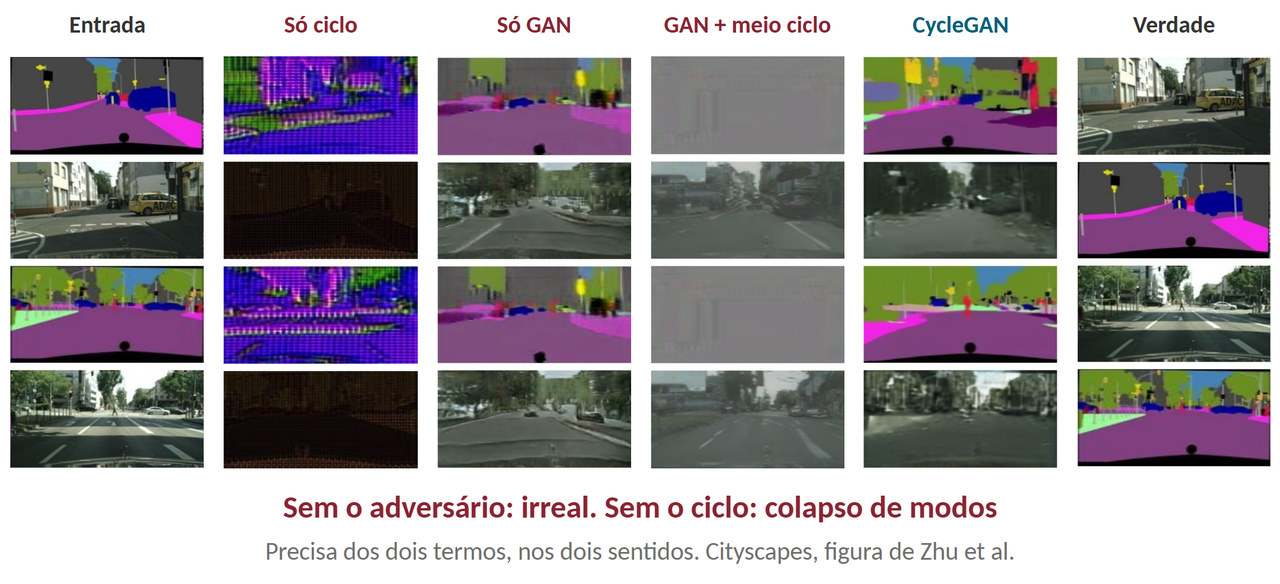
\includegraphics[width=124.4mm]{f_ablacao}
  \fonte{Zhu et al. 2017, fig. 7, em DeepLearning.AI C3W3}
\end{frame}

\section{Aplicações e o nosso exemplo}
\begin{frame}{Roteiro}
  \vspace{4mm}
    {\small\textcolor{coppeGray}{{1. Como uma GAN funciona}}}\par\smallskip
    {\small\textcolor{coppeGray}{{2. Problemas na dinâmica adversarial}}}\par\smallskip
    {\small\textcolor{coppeGray}{{3. Controlar e avaliar}}}\par\smallskip
    {\small\textcolor{coppeGray}{{4. StyleGAN}}}\par\smallskip
    {\small\textcolor{coppeGray}{{5. Pix2Pix e CycleGAN}}}\par\smallskip
    {\small\textcolor{coppeAccent}{\textbf{6. Aplicações e o nosso exemplo}}}\par\smallskip
    {\footnotesize\textcolor{coppeGray}{Imagem, áudio, medicina e, no fim, o que nós rodamos: Pokémon}}\par\smallskip
\end{frame}

\begin{frame}{GAN não é só imagem}
  \centering
  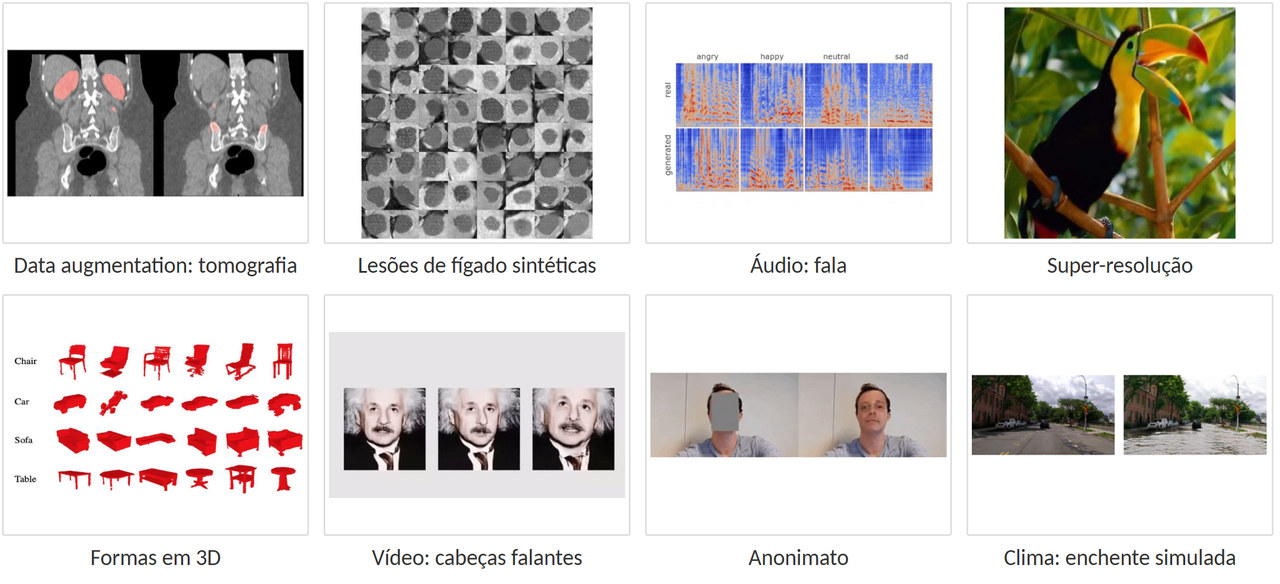
\includegraphics[width=124.4mm]{f_aplic}
  \fonte{DeepLearning.AI C1W1 e C3W1, com as fontes originais em S62}
\end{frame}

\begin{frame}{GAN, VAE e difusão}
  \centering
  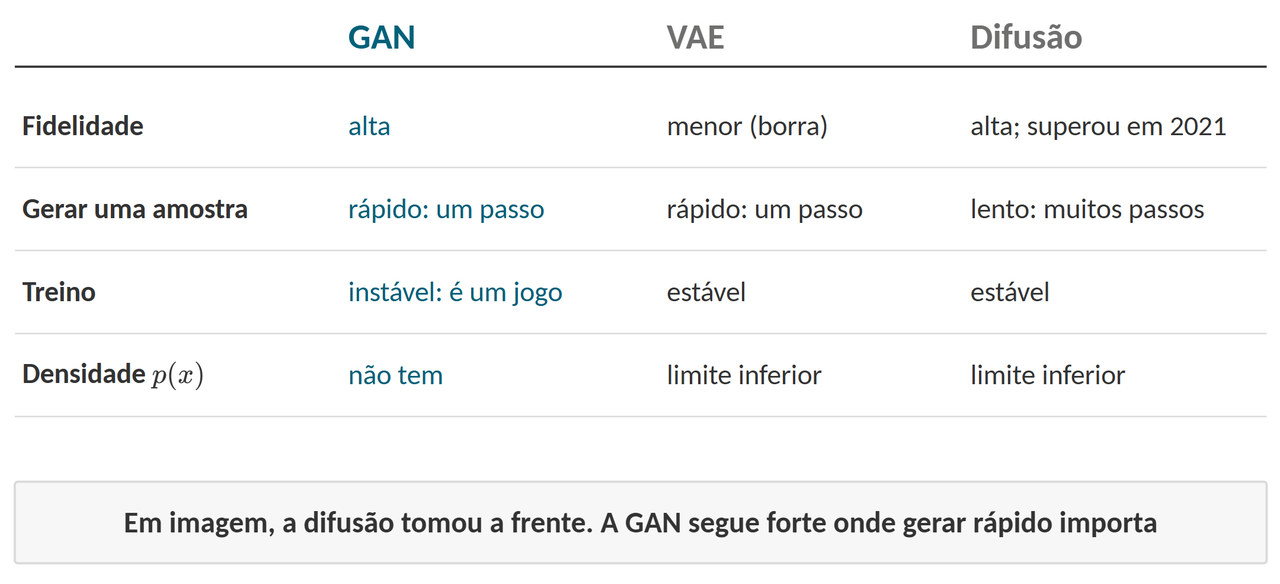
\includegraphics[width=124.4mm]{f_comparar}
  \fonte{DeepLearning.AI C2W2 \textperiodcentered{} Dhariwal e Nichol 2021}
\end{frame}

\begin{frame}{Nosso exemplo: Pokémon}
  \centering
  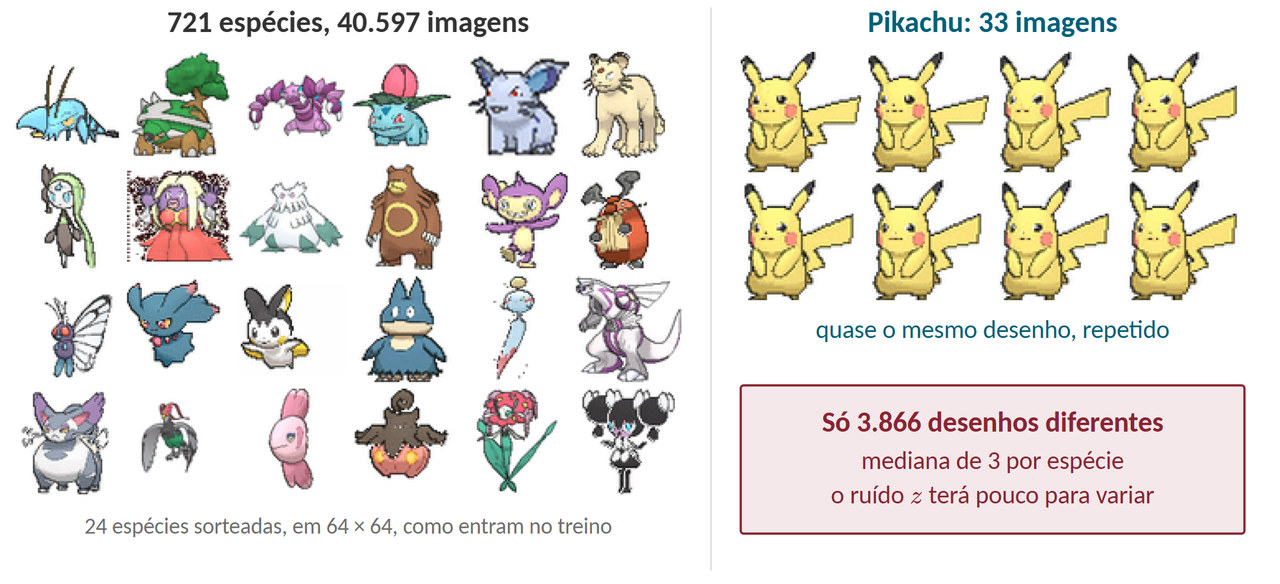
\includegraphics[width=124.4mm]{f_pk_dados}
  \fonte{Sprites: Zhang et al., Dive into Deep Learning, cap. 20 (d2l.ai) \textperiodcentered{} nosso: exemplos/pokemon}
\end{frame}

\begin{frame}{Os problemas, na prática}
  \centering
  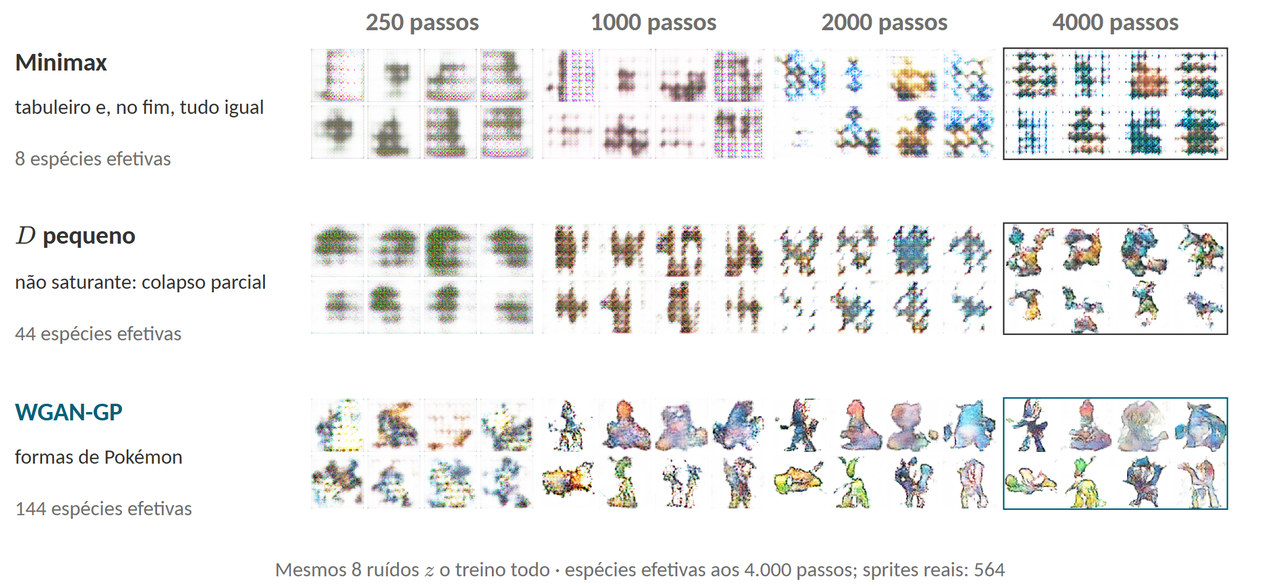
\includegraphics[width=124.4mm]{f_pk_evolucao}
  \fonte{Nosso: a mesma DCGAN, 4.000 passos por perda \textperiodcentered{} $D$ pequeno: receita de Metz et al. 2016}
\end{frame}

\begin{frame}{Vanishing gradient, medido}
  \centering
  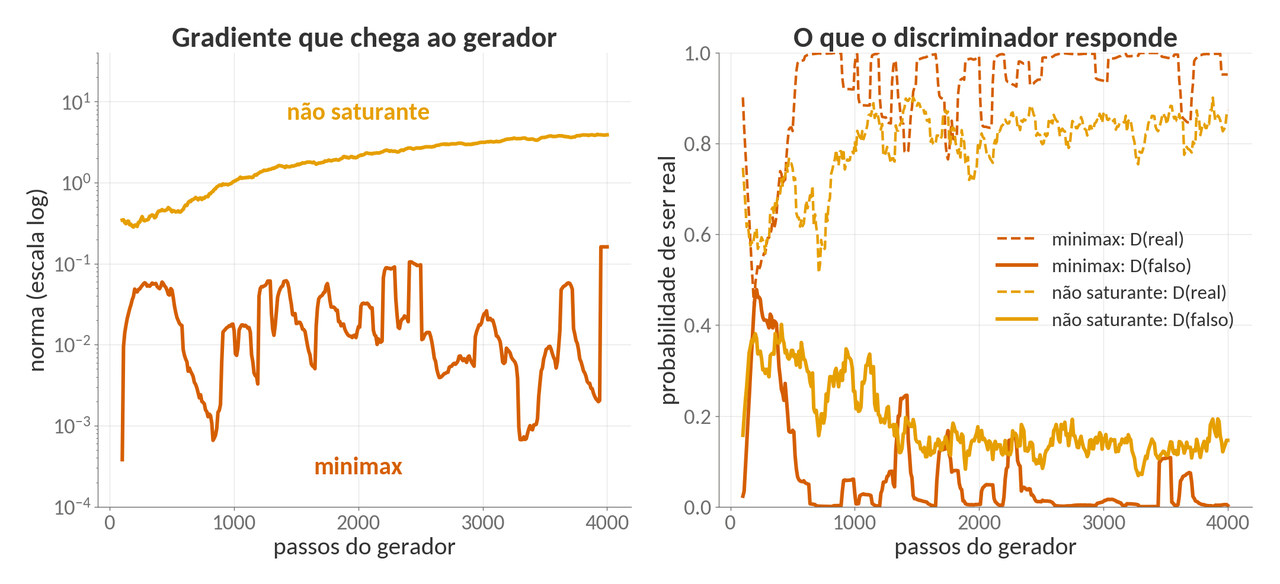
\includegraphics[width=124.4mm]{f_pk_gradiente}
  \fonte{Nosso \textperiodcentered{} média móvel de 10 registros}
\end{frame}

\begin{frame}{Qual treino vai melhor?}
  \centering
  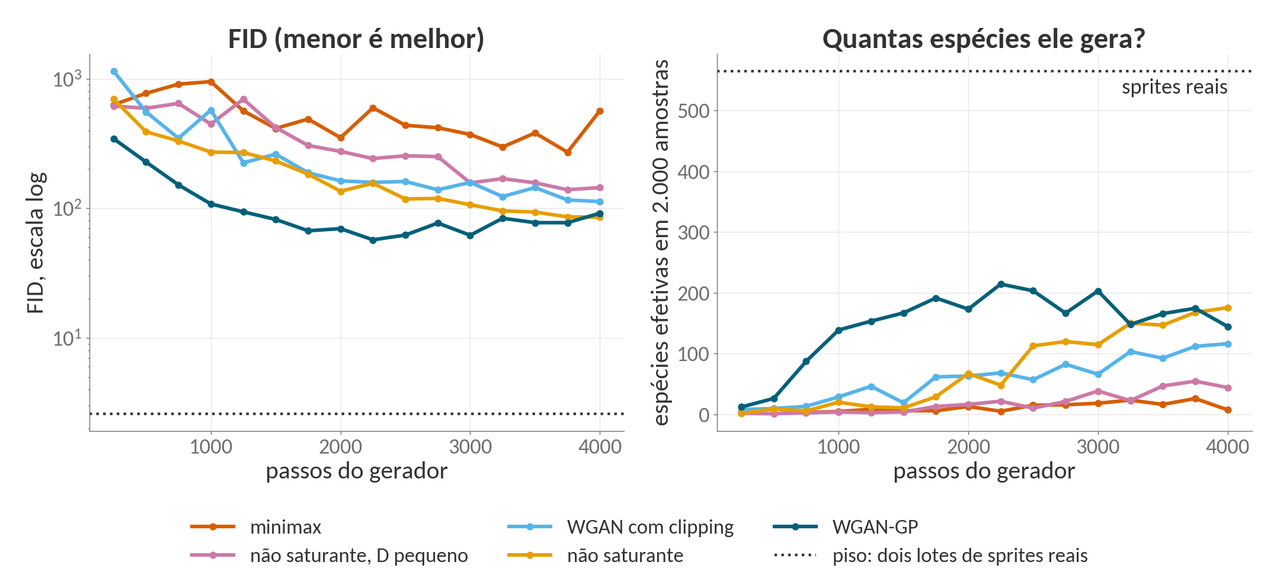
\includegraphics[width=124.4mm]{f_pk_fid}
  \fonte{Nosso \textperiodcentered{} FID e espécies nos atributos de um classificador de espécies treinado nos sprites reais}
\end{frame}

\begin{frame}{A nota do crítico}
  \centering
  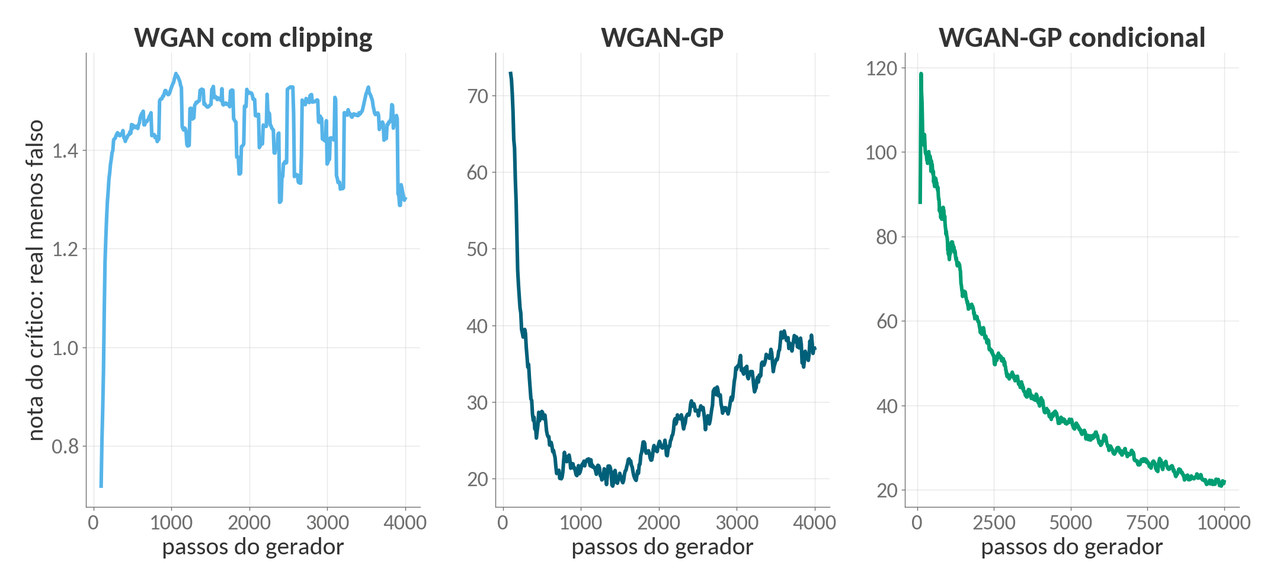
\includegraphics[width=124.4mm]{f_pk_wasserstein}
  \fonte{Nosso \textperiodcentered{} média móvel de 10 registros}
\end{frame}

\begin{frame}{Nossa StyleGAN para Pokémon}
  \centering
  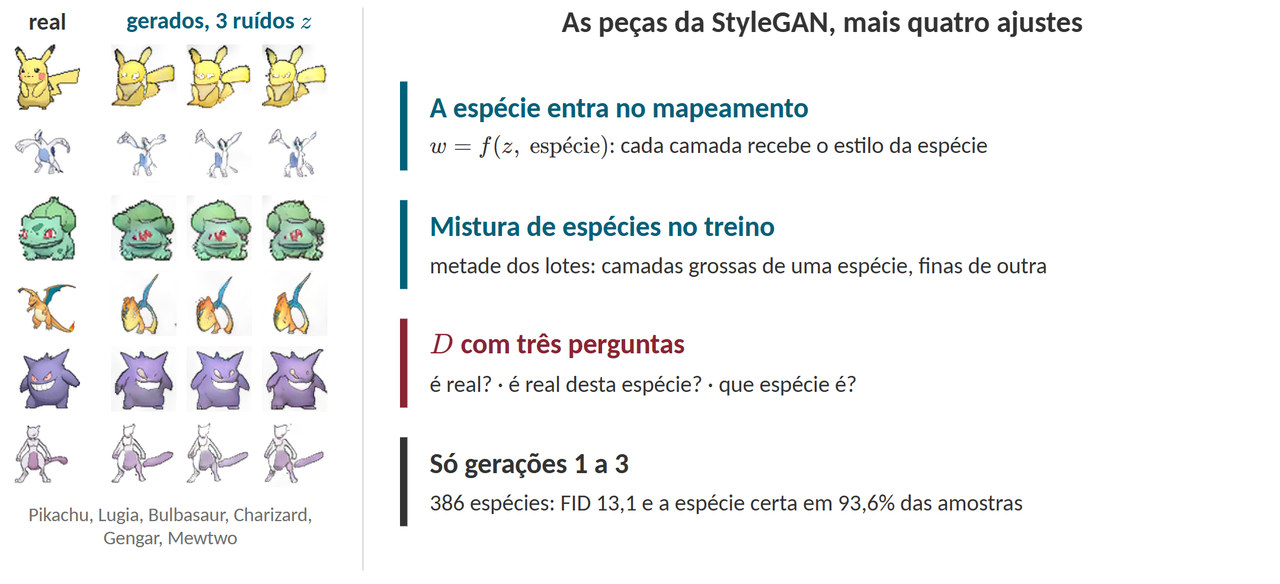
\includegraphics[width=124.4mm]{f_pk_arq}
  \fonte{Nosso: exemplos/pokemon/estilo\_gan.py \textperiodcentered{} base: Karras et al. 2020 \textperiodcentered{} $D$: Miyato e Koyama 2018, Odena et al. 2017 \textperiodcentered{} Shahbazi et al. 2022}
\end{frame}

\begin{frame}{O treino da nossa StyleGAN}
  \centering
  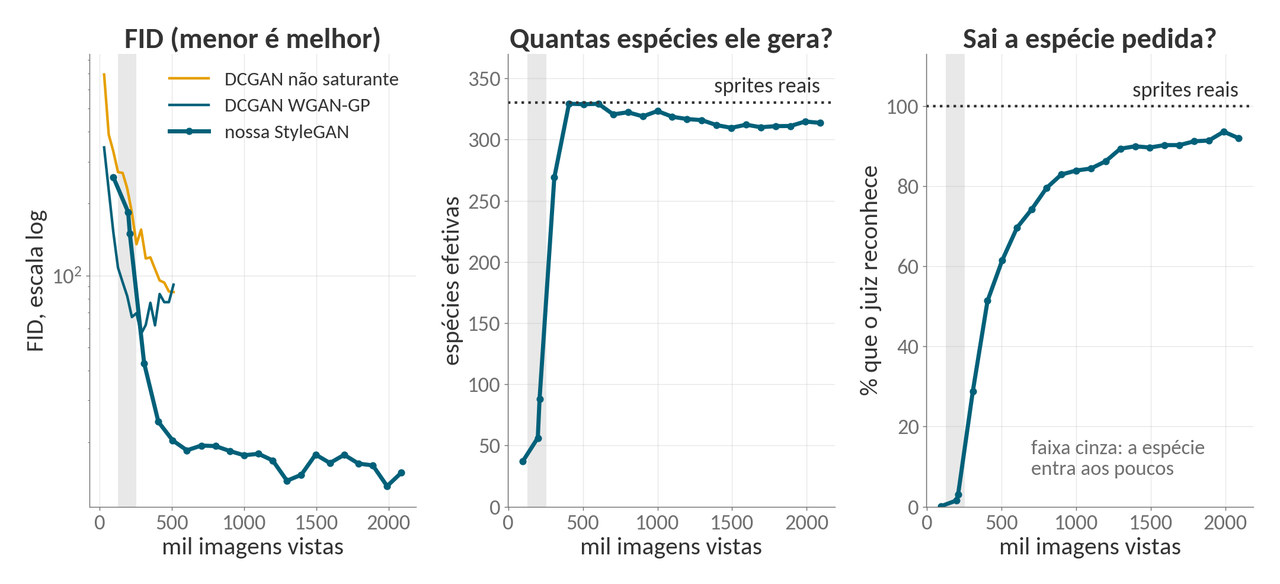
\includegraphics[width=124.4mm]{f_pk_curvas}
  \fonte{Nosso: 2,1 milhões de imagens, 5,6 h numa RTX 2060 \textperiodcentered{} transição da espécie: Shahbazi et al. 2022}
\end{frame}

\begin{frame}{Pikachugia e Lugachu}
  \centering
  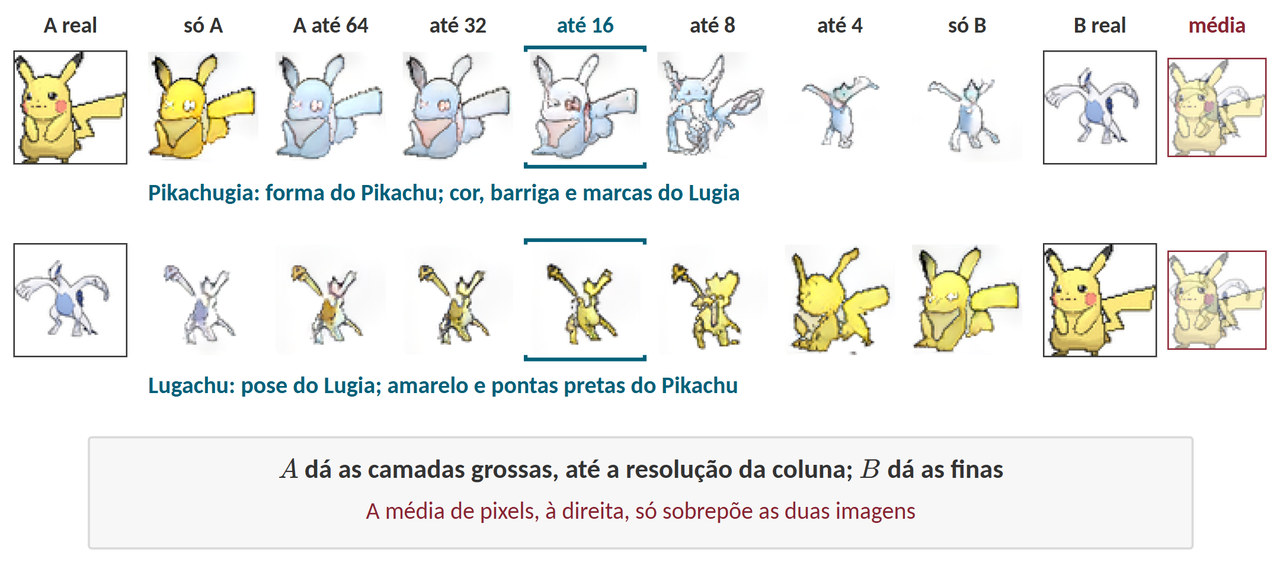
\includegraphics[width=124.4mm]{f_pk_ponte}
  \fonte{Nosso \textperiodcentered{} mistura de estilos como em Karras et al. 2018, fig. 3}
\end{frame}

\begin{frame}{Qualquer par de espécies}
  \centering
  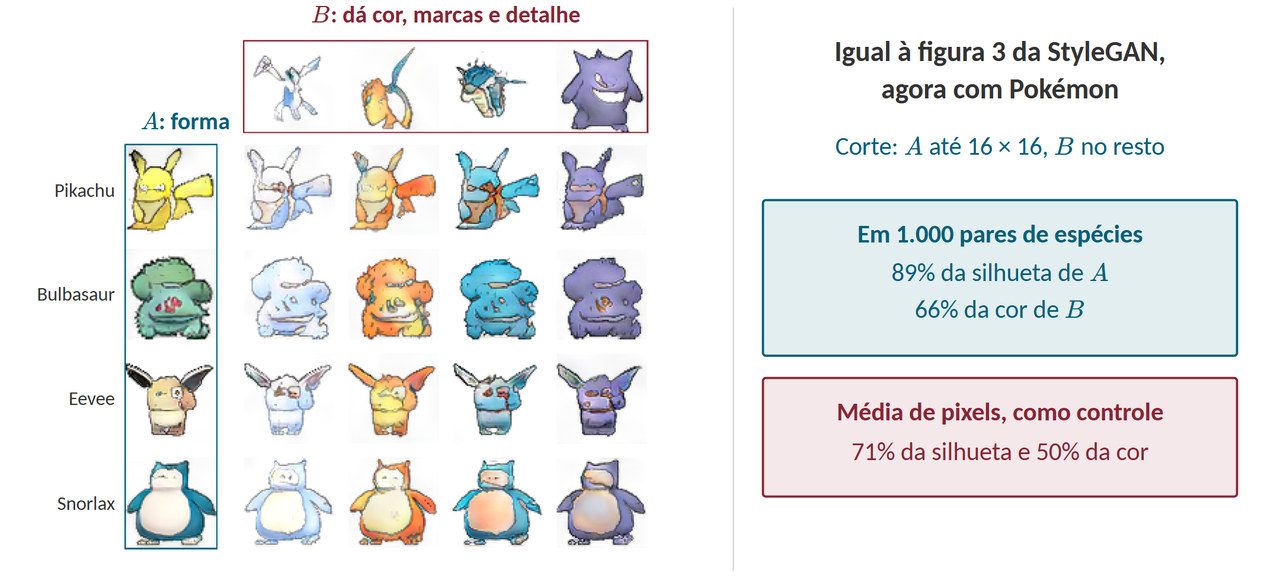
\includegraphics[width=124.4mm]{f_pk_pares}
  \fonte{Nosso \textperiodcentered{} como em Karras et al. 2018, fig. 3}
\end{frame}

\begin{frame}{A ponte, medida}
  \centering
  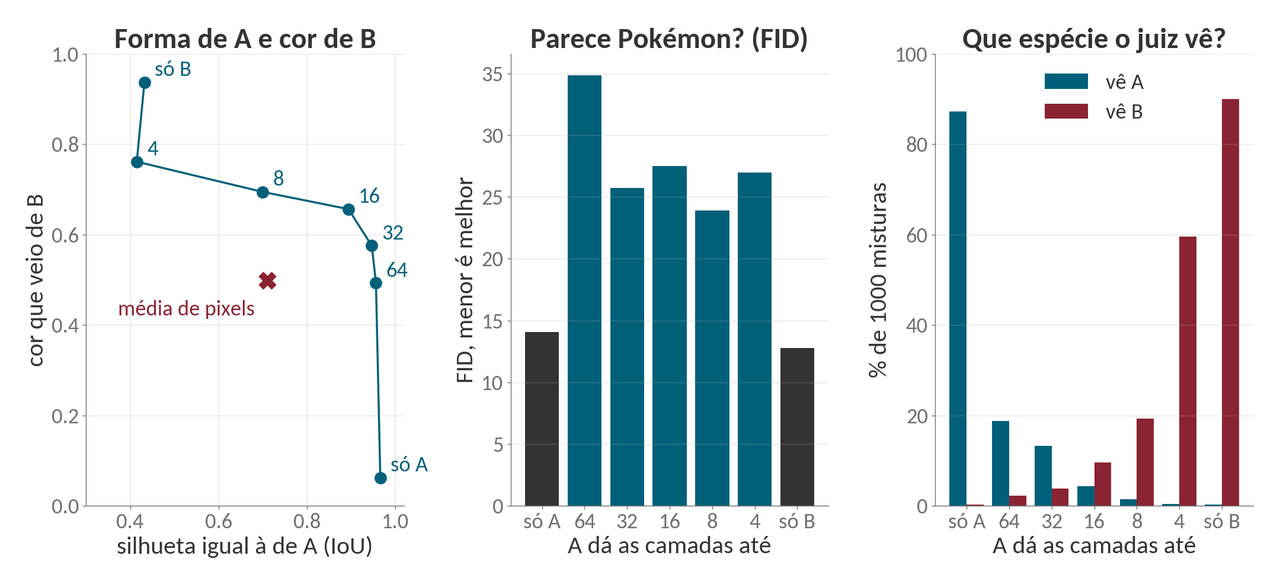
\includegraphics[width=124.4mm]{f_pk_medidas}
  \fonte{Nosso, 1.000 pares de espécies \textperiodcentered{} o juiz é o classificador de espécies, que não entra no treino}
\end{frame}

\begin{frame}{O que o exemplo ensinou}
  \centering
  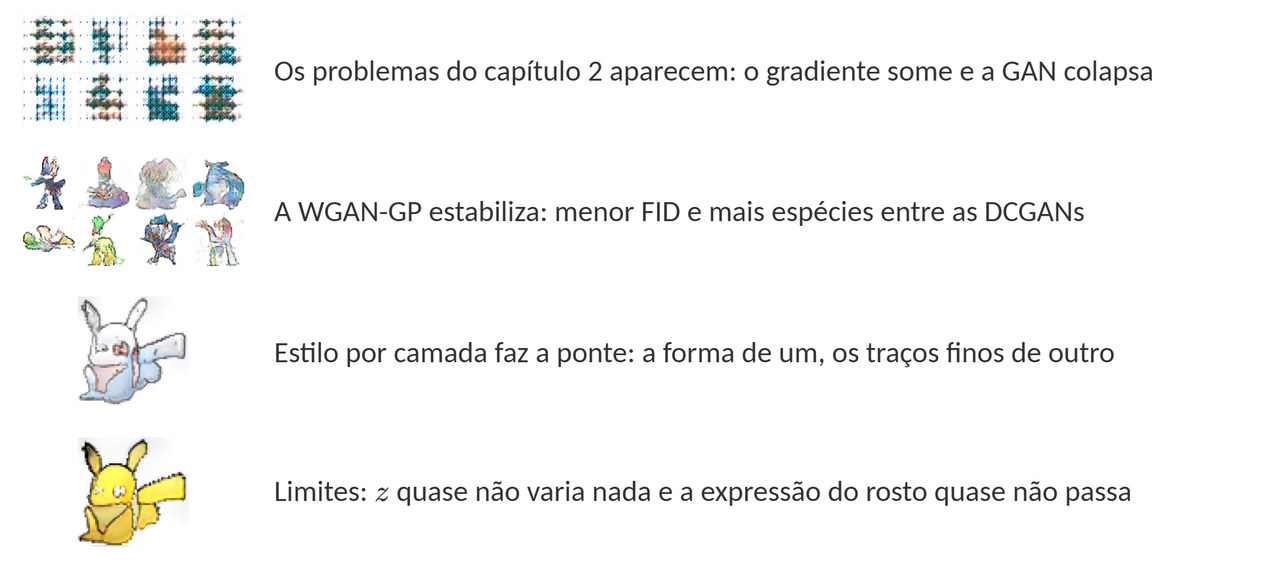
\includegraphics[width=124.4mm]{f_pk_licoes}
  \fonte{Nosso}
\end{frame}

\begin{frame}{Para levar}
  \centering
  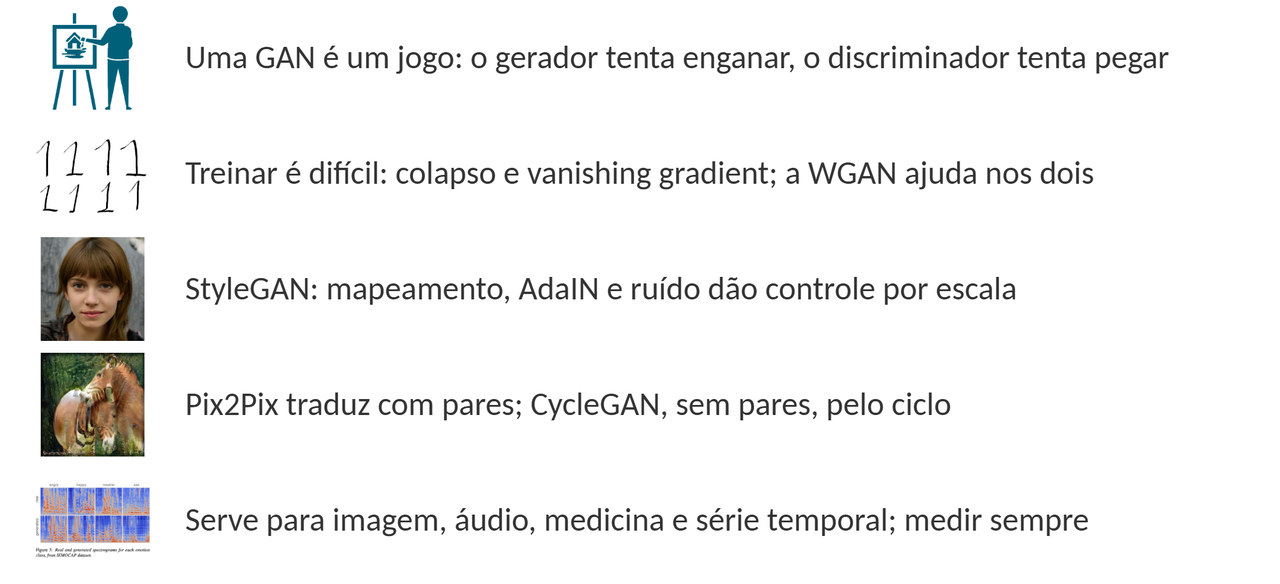
\includegraphics[width=124.4mm]{f_fecho}
\end{frame}

\appendix
\section*{Apoio}

\begin{frame}{Apoio: a conta do D ótimo e da JS}
  \centering
  \resizebox{79.1mm}{!}{$\displaystyle V(G,D)=\int_x\Big[p_{\text{dados}}(x)\log D(x)+p_g(x)\log\big(1-D(x)\big)\Big]dx$}\par\vspace{1.5mm}
  \resizebox{80.1mm}{!}{$\displaystyle \frac{d}{dy}\big[a\log y+b\log(1-y)\big]=\frac{a}{y}-\frac{b}{1-y}=0\ \Longrightarrow\ y^{*}=\frac{a}{a+b}$}\par\vspace{1.5mm}
  \resizebox{83.4mm}{!}{$\displaystyle \max_D V=\mathbb{E}_{p_{\text{dados}}}\log\frac{p_{\text{dados}}}{2m}+\mathbb{E}_{p_g}\log\frac{p_g}{2m},\qquad m=\tfrac12(p_{\text{dados}}+p_g)$}\par\vspace{1.5mm}
  \resizebox{87.7mm}{!}{$\displaystyle =-\log 4+\mathrm{KL}(p_{\text{dados}}\Vert m)+\mathrm{KL}(p_g\Vert m)=-\log 4+2\,\mathrm{JS}(p_{\text{dados}}\Vert p_g)$}\par\vspace{1.5mm}
  \fonte{Goodfellow et al. 2014, prop. 1 e teo. 1}
\end{frame}

\begin{frame}{Apoio: referências}
  \begin{columns}[T,onlytextwidth]
    \begin{column}{0.48\textwidth}\raggedright\tiny
      Goodfellow, Bengio, Courville (2016). Deep Learning, cap. 20\par\smallskip
      DeepLearning.AI. GANs Specialization (slides, CC BY-SA 2.0)\par\smallskip
      Goodfellow et al. (2014) 1406.2661 \textperiodcentered{} tutorial (2016) 1701.00160\par\smallskip
      Radford et al. (2015) DCGAN 1511.06434\par\smallskip
      Mirza, Osindero (2014) cGAN 1411.1784\par\smallskip
      Arjovsky, Bottou (2017) 1701.04862\par\smallskip
      Arjovsky et al. (2017) WGAN 1701.07875\par\smallskip
      Gulrajani et al. (2017) WGAN-GP 1704.00028\par\smallskip
      Mao et al. (2016) LSGAN 1611.04076\par\smallskip
      Heusel et al. (2017) FID 1706.08500\par\smallskip
      Kynkäänniemi et al. (2019) 1904.06991\par\smallskip
    \end{column}
    \begin{column}{0.48\textwidth}\raggedright\tiny
      Karras et al. (2017) ProGAN 1710.10196\par\smallskip
      Brock et al. (2018) BigGAN 1809.11096\par\smallskip
      Karras et al. (2018) StyleGAN 1812.04948\par\smallskip
      Karras et al. (2019) StyleGAN2 1912.04958\par\smallskip
      Karras et al. (2021) StyleGAN3 2106.12423\par\smallskip
      Sauer et al. (2022) StyleGAN-XL 2202.00273\par\smallskip
      Kang et al. (2023) GigaGAN 2303.05511\par\smallskip
      Pan et al. (2023) DragGAN 2305.10973\par\smallskip
      Huang et al. (2025) R3GAN 2501.05441\par\smallskip
      Dhariwal, Nichol (2021) 2105.05233\par\smallskip
      Isola et al. (2016) Pix2Pix 1611.07004\par\smallskip
      Zhu et al. (2017) CycleGAN 1703.10593\par\smallskip
      \textbf{No nosso exemplo:} Zhang et al. Dive into Deep Learning, cap. 20 (d2l.ai)\par\smallskip
      Karras et al. (2020) StyleGAN2-ADA 2006.06676\par\smallskip
      Odena et al. (2017) AC-GAN 1610.09585 \textperiodcentered{} Miyato, Koyama (2018) 1802.05637\par\smallskip
      Shahbazi et al. (2022) 2201.06578 \textperiodcentered{} Metz et al. (2016) 1611.02163\par\smallskip
      Zhao et al. (2020) DiffAugment 2006.10738 \textperiodcentered{} Mescheder et al. (2018) 1801.04406\par\smallskip
    \end{column}
  \end{columns}
\end{frame}

\begin{frame}{Apoio: créditos das imagens}
  \begin{columns}[T,onlytextwidth]
    \begin{column}{0.48\textwidth}\raggedright\tiny
      Silhuetas, Mona Lisa, gatos, dígitos manuscritos, cabelo: DeepLearning.AI, cursos 1 e 2, CC BY-SA 2.0\par\smallskip
      Rostos: Karras et al. 2018 e 2020, via curso\par\smallskip
      Tweet: I. Goodfellow, via curso C2W3\par\smallskip
      Truncamento: Brock et al. 2018\par\smallskip
      Precisão e revocação: Kynkäänniemi et al. 2019\par\smallskip
    \end{column}
    \begin{column}{0.48\textwidth}\raggedright\tiny
      Pix2Pix, GauGAN: Isola et al. 2016, Park et al. 2019, via curso C3W2\par\smallskip
      CycleGAN: Zhu et al. 2017 e togheppi/CycleGAN, via curso C3W3\par\smallskip
      Fígado: arXiv:1803.01229; tomografia: Nature Sci. Rep., s41598-019-52737-x; via curso C3W1\par\smallskip
      Onda e huskies: DeepLearning.AI, cursos C1W3 e C1W4\par\smallskip
      Quartos, interpolação e aritmética em $z$: Radford et al. 2015, fig. 3, 4 e 7\par\smallskip
      Discriminador e crítico em 1D: Arjovsky et al. 2017, fig. 2\par\smallskip
      Amostras condicionais: Brock et al. 2018, fig. 1\par\smallskip
      Sprites de Pokémon: Zhang et al., Dive into Deep Learning\par\smallskip
      Treinos, curvas e misturas de Pokémon: nossos\par\smallskip
      Todo o resto: diagramas nossos\par\smallskip
    \end{column}
  \end{columns}
\end{frame}

\end{document}
